%D�finir le format du document: papier, taille de police, type de document, etc.
\documentclass[a4paper, 11pt]{article}

%%%%%%%%% Packages externes utilis�s %%%%%%%%%%%%%%%%%%%
\usepackage[french]{babel}
\usepackage[latin1]{inputenc}
\usepackage[T1]{fontenc}
\usepackage{verbatim}
\usepackage{graphicx}
\usepackage{epstopdf}
\usepackage{macro}
\usepackage{algorithm}
\usepackage{algorithmic}
%\usepackage{algorithm2e}


%La mise en page du rapport, NE PAS MODIFIER.
\usepackage{geometry}
 \geometry{
 a4paper,
 left=20mm,
 right=20mm,
 top=20mm,
 bottom=20mm,
 }

%%%%%%%%% Le corps du document entre begin et end %%%%%%%%%%%%%%%%%%%
\begin{document}

%Page de garde
%%%%%%%%%%%%%%% Page de garde %%%%%%%%%%%%%%%%%%%

\begin{titlepage}{
    \begin{center}
        \vspace* {25mm}
        {\Large \textbf {Universit� de Cergy-Pontoise}} \\
        \vspace* {10mm}
        {\Large \textbf {RAPPORT}} \\
        \vspace* {10mm}
        pour le projet G�nie Logiciel \\
        \textbf {Licence d'Informatique deuxi�me ann�e} \\
        \vspace* {10mm}

	sur le sujet \\
        \vspace* {10mm}
	{\Huge \textsf{Urbain}} \\
        \vspace* {10mm}
 	r�dig� par \\
        \vspace* {10mm}
        {\Large \textbf {Matthieu VILAIN et Quentin GERARD}} \\
				\vspace* {10mm}
				\noreffig{images/ville.png}{12.82cm}{8.2cm} \\
        \date Mai 2015
        \vspace* {10mm}
	\end{center}
}
\end{titlepage}

%G�n�ration automatique de la table des mati�res, de la liste des figures et de la liste des tableaux
\tableofcontents

%Une section "remerciements" pourrait �tre int�ressante. C'est une section non num�rot� (avec un * )
\section*{Remerciements}
Les auteurs du projet voudraient remercier...

\section{Introduction}
\label{sec:introduction}

\paragraph{Le projet}
Le projet consiste � la cr�ation d'un jeu vid�o simulant une vie urbaine, dans laquelle
plusieurs individus vivent leur vie au sein d'une ville. L'utilisateur pourra infuer sur le comportement
des individus et les param�tres de la ville.

\paragraph{Fonctionnalit�s} Fonctionnalit�s du programme:
Le joueur aura plusieurs actions possibles afn d'infuer sur l'�volution de la ville. Tout
d'abord il pourra agir sur le temps en l?acc�l�rant ou en le mettant en pause. Ensuite il pourra acc�der
� des informations sur les personnages comme : leurs informations de bases, leur historique ou leurs
objectifs directs (exemple : ce personnage se rend � la piscine). Ces informations pourront �tre
chang�es par l'utilisateur et il pourra ainsi renommer un personnage, le faire d�m�nager ou le faire
rentrer chez lui par exemple. De m�me pour les b�timents, l'utilisateur pourra acc�der � ses
informations et les modifer. Il pourra donc par exemple modifer les horaires d'ouverture d'un lieu ou
faire varier son nombre d'utilisateur maximum. Le joueur pourra donc modifer � sa guise ses
informations et voir ce que ces modifcations apportent de bon ou de mauvais sur � population de la
ville.

\paragraph{Nos motivations}
Nous avons choisi ce projet car il repr�sente une opportunit� pour chacun de nous
d?explorer des domaines/notions qui nous int�ressent, et dans lesquelles nous voulons nous
perfectionner.

\section{Sp�cification}
\label{sec:specification}

\paragraph{Chapeau} Nous avons pr�sent� l'objectif du projet dans la section \ref{sec:introduction}. Dans cette section, nous pr�sentons la sp�cification de notre logiciel r�alis�. Ceci correspond principalement au cahier des charges.

\subsection{Premi�re sous-section}
\label{sec:spec1}

\paragraph{Premier paragraphe} On commence � expliquer...

\paragraph{} Juste un simple paragraphe.

\subsection{Deuxi�me sous-section}
\label{sec:spec2}

\begin{table}[h!]
\centering
\begin{tabular} {|p{3.5cm}|p{2.5cm}|p{5cm}|}
\hline
Document & Coefficient & Commentaire \\
\hline
Cahier des charges & 37.5\% & Premier document \\
\hline
Rapport & 62.5\% & Rapport final du projet \\
\hline
\end{tabular}
\caption{Documents � remettre}
\label{tab:document}
\end{table}

Comme ce qui est illustr� dans le tableau \ref{tab:document}, ...

\section{R�alisation}
\label{sec:impl}

%\begin{figure}
%\centering
%
\includegraphics[width=3.5cm, height=2cm]{images/programmer.png}
%\caption{Un programmeur occup�}
%\label{fig:modele}
%\end{figure}

\subsection{Le Model - pr�sentation des classes}

\subsubsection{La ville}

La ville est le premier �l�ment qui constitue notre projet. Elle est compos�e de diff�rentes infrastructures�: Les routes, les maisons, les b�timents de travail et les divertissements. Chaque type d'infrastructure poss�de une utilit� qui lui est propre�:
\begin{itemize}
 \item Les Routes permettent aux personnages de se d�placer
 \item Les Maisons permettent aux personnages de se reposer le soir et regagner de l'�motion
 \item Le Travail est une activit� impos� � chaque personnages et sera la principale source de baisse d'�motion
 \item Les Divertissements permettent aux personnages lorsqu'ils ne dorment pas de regagner de l'�motion
\end{itemize}

#image

\paragraph{}
Toutes les infrastructures poss�dent en commun�: 
\begin{itemize}
 \item Un nom de type String
 \item Un type au format int
 \item Une position dans la Map
 \item Un taille
 \item Et un nombre d'utilisateurs courant
\end{itemize}

 \paragraph{}
 Et les b�timents (hors routes) poss�dent tous en commun ces caract�ristiques�:
 \begin{itemize}
  \item Une adresse, seule point d'entr� dans le b�timents au niveau de la Map
  \item Une r�compense, qui peut �tre positive ou n�gative suivant le type de b�timent
  \item Un nombre maximum d'utilisateur 
 \end{itemize}
 
 \paragraph{}
En plus de ces caract�ristiques, les b�timents de travail et les divertissements poss�dent un temps d'utilisation moyen par les personnages, ainsi que des horaires d'ouvertures durant lesquelles les personnages pourront utiliser ces b�timents. 
Il est �galement impossible pour un personnages d'utiliser un b�timent lorsque celui ci � atteint son nombre maximum d'utilisateur.
Les routes et les maisons sont ouverts 24h/24.

\paragraph{}
La taille de la Map ainsi que la r�partition des infrastructures est d�termin� � l'avance dans un fichier CSV. La cr�ation de la Map dans la m�moire se fait gr�ce au design pattern Builder. 
Chaque ligne du fichier CSV renseigne, le type, l'adresse, la taille et sa position dans la Map. 
Ainsi l'objet MapBuilder va lire les lignes du fichier une par une gr�ce � la biblioth�que Apache Common CSV, et faire appelle au autres Builder correspondant � chaque type d'infrastructure.
 
 \paragraph{}
 Durant leur cr�ation, les Infrastructures de type Work ou Entertainement, se voient �galement attribuer un nom, des horaires d'ouvertures et leur r�compenses. 
 Ces informations sont aussi renseign�es � l'avance dans un fichier CSV.
 
 \subsubsection{La population}
 
 \paragraph{}
 La population est le second ensemble qui constitue notre projet. 
 Nous l'avons voulu le plus adaptatif possible. 
 Ainsi elle peut contenir autant d'individu que souhait�. 
 Cependant, une trop grande population provoquera des ralentissements de l'interface graphique mais le moteur de jeu est parfaitement capable de faire tourner une grande population. 
 Pour la jouabilit� du jeu, nous avons fix� le nombre d'individus au d�marrage d'une partie � 5. 
 
 \paragraph{Cr�ation des personnages}
 Un personnage est compos� d'informations de base comme d'un nom, d'un pr�nom, d'un sexe , d'un age et d'un num�ro d'identit�.

 \fig{images/car.jpg}{8cm}{7cm}{Classe Character}{characterClass}
 
 \paragraph{}
 Pour le nom, le pr�nom et le sexe du personnage, ils sont initialis�s � partir de fichier CSV. 
 Le premier fichier contient une liste de 300 noms de familles et le second une liste de 200 pr�noms, 100 masculin et 100 f�minin. 
 Lors de la cr�ation du personnage, le programme va prendre au hasard un nom dans le fichier name.csv et un pr�nom (associ� � un sexe) dans le fichier firstName.csv. 
 L'age du personnage est simplement choisit al�atoirement entre 10 et 100 ans. 
 Le num�ro d'identit� du personnage est unique, il est calcul� � partir de toutes les informations du personnage gr�ce � un code de hashage. 
 Ce code nous permettra de reconna�tre le personnage. 
 Ce grand nombre de choix nous permet de garantire une grande diversit� au sein de la population.
 
 \paragraph{}
  Comme le montre la figure 1, un personnage poss�de �galement une maison et un travail. 
  Ces deux �l�ments sont �galement attribu� al�atoirement via une recherche dans la liste de lieux de travail et d'habitation de la carte de jeu.
  
 \paragraph{}
 Un personnage poss�de �galement une jauge d'�motion qui peut varier de 0 � 100. 
 C'est comme la barre de vie du personnage. 
 Elle est initialis� a 75 en d�but de partie mais elle variera en fonctions des actions des personnages. 
 Si le personnage atteint une �motion de 0 il meurt.
 
 \paragraph{}
 Enfin la cr�ation de la routine sera expliqu� dans la partie moteur.
 
 \paragraph{}
 Nous avons voulu rendre nos personnages le moins statique possible. Ainsi d'une partie � l'autre, la chance de tomber sur des personnages avec les m�mes propri�t�s est tr�s faible.
 
 \paragraph{L'organisation de la cr�ation}
 des personnages se fait gr�ce au design pattern builder.
 
 \begin{figure}[!h] 	
  \centering 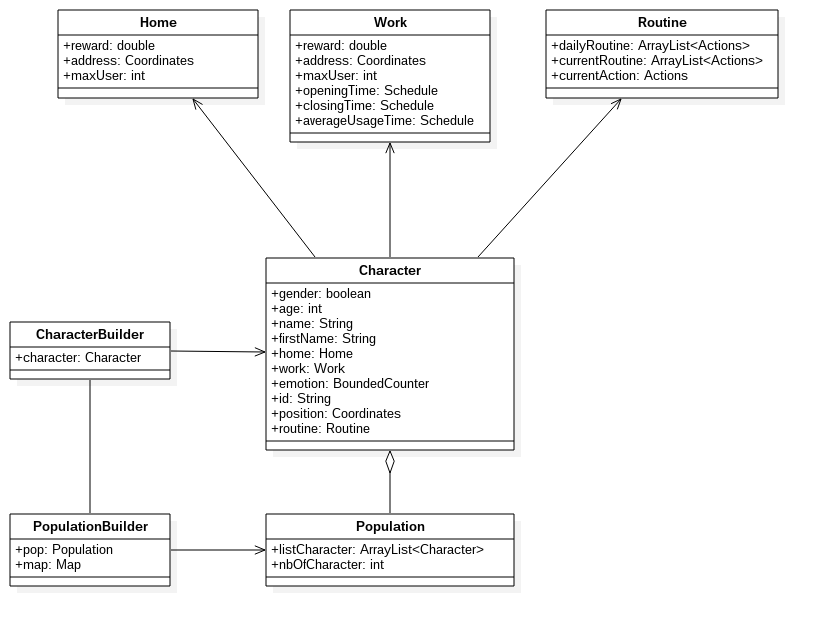
\includegraphics[width=400pt]{images/pop.png}
  \caption{Organisation de la partie population} \label{fig:population}
\end{figure}
 
 \paragraph{}
 La classe PopulationBuilder va construire une population gr�ce � la carte de jeu (pour assigner les r�sidences) et gr�ce au CharacterBuilder. 
 Ce dernier va faire la lecture dans les fichiers CSV gr�ce � la biblioth�que Apache-commons-csv et va faire les choix al�atoires pour initialiser les diff�rentes composantes de nos personnages.
 
 \subsection{Le moteur de jeu}
 
 \subsubsection{Gestion de l'�motion des personnages}
 
 \paragraph{}
 L'�motion repr�sente la barre de vie des personnages, elle varie de 0 � 100 en fonction du temps. 
 Si elle atteint 0, le personnage meurt. 
 L?�volution de cette jauge d?�motion est totalement dynamique, elle se fera automatiquement en fonction des actions faites par le personnage. 
 Certaines actions vont apporter un bonus sur la jauge d'�motion du personnage alors que d'autres vont apporter un malus. 
 Pour certaines actions le bonus est constant (par exemple dormir apportera toujours +30) mais pour d'autres le bonus/malus est variable en fonction du lieu dans lequel se fait l'action. 
 Par exemple travailler dans un atelier auto apportera un malus de -25 car la tache est difficile alors que travailler dans une boutique d?�lectronique apportera un malus de -15. 
 M�me fonctionnement pour les bonus des loisirs. 
 Ces valeurs sont initialiser lors que l'initialisation des b�timents, elles proviennent donc d'un fichiers CSV. 
 Enfin les rewards de sont pas toujours effectif au m�me moment. 
 Pour la plupart des actions, le personnage per�oit le reward en fin d'action. 
 Pour l'action de d�placement, dans un soucis de mieux repr�senter la r�alit�, le malus est retir� � chaque it�ration de temps. 
 C'est � dire que plus le chemin que le personnage a � faire est long, plus il perd de l'�motion.
 
 \begin{tabular} {|p{3.5cm}|p{5cm}|p{5cm}|}
\hline
Action & Reward & Effectivit� \\
\hline
Sleeping & +30 & En fin d'action \\
\hline
Chilling & +5 & En fin d'action \\
\hline
Schifting & -1 & A chaque it�ration de temps \\
\hline
Working & Malus variable [-25;-10] & En fin d'action \\
\hline
Entertain & Bonus variable [+5;+20] & En fin d'action \\
\hline
\end{tabular}

\subsubsection{Gestion de la routine}
\paragraph{}
La routine est un encha�nement d'actions que va ex�cuter le personnage. 
Le personnage peut ex�cuter 5 types d'actions diff�rentes regrouper en familles�: les d�placements et les occupations.  
Les actions d'occupation sont reli�es � un lieu alors que les actions de d�placement sont reli�es � un lieu de d�part, un lieu d'arriv� et un chemin entre les deux.


\begin{figure}[!h] 	
  \centering 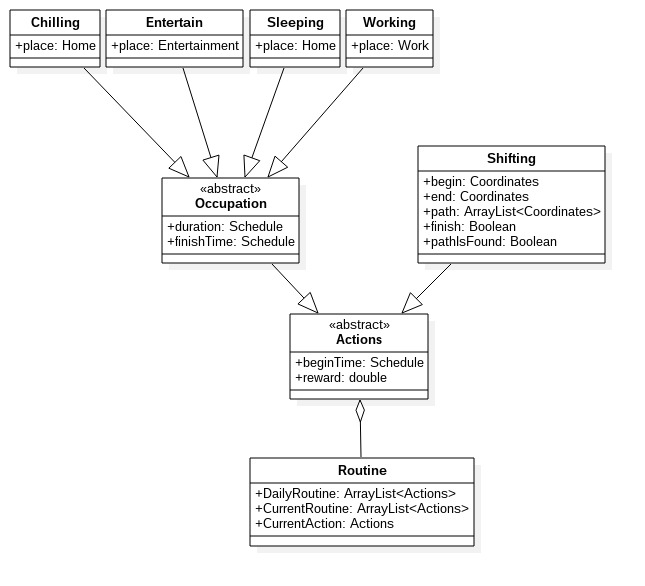
\includegraphics[width=400pt]{images/routine.jpg}
  \caption{Classe routine} \label{fig:characterClass}
\end{figure}

\paragraph{}
L'un des dilemme du projet est l?interaction entre les diff�rentes actions pour  que chaque personnage puisse avoir puisse suivre une suite d'actions ind�pendantes mais que l'utilisateur puisse ajouter des actions a faire sans perturber le bonne encha�nement des actions.

\paragraph{}
Nous avons d�cid� de d�composer ce probl�me en 3 partie�:
\begin{itemize}
 \item Une partie statique qui organise les grandes lignes des journ�es du personnage�: m�tro/boulot/dodo
 \item Une partie dynamique qui �volue au court de la journ�e et qui repr�sente la liste d'actions que le personnage a � faire
 \item Une partie utilisateur associ� � diff�rente options d'ajout/suppression d'actions 
\end{itemize}

\begin{figure}[!h] 	
  \centering 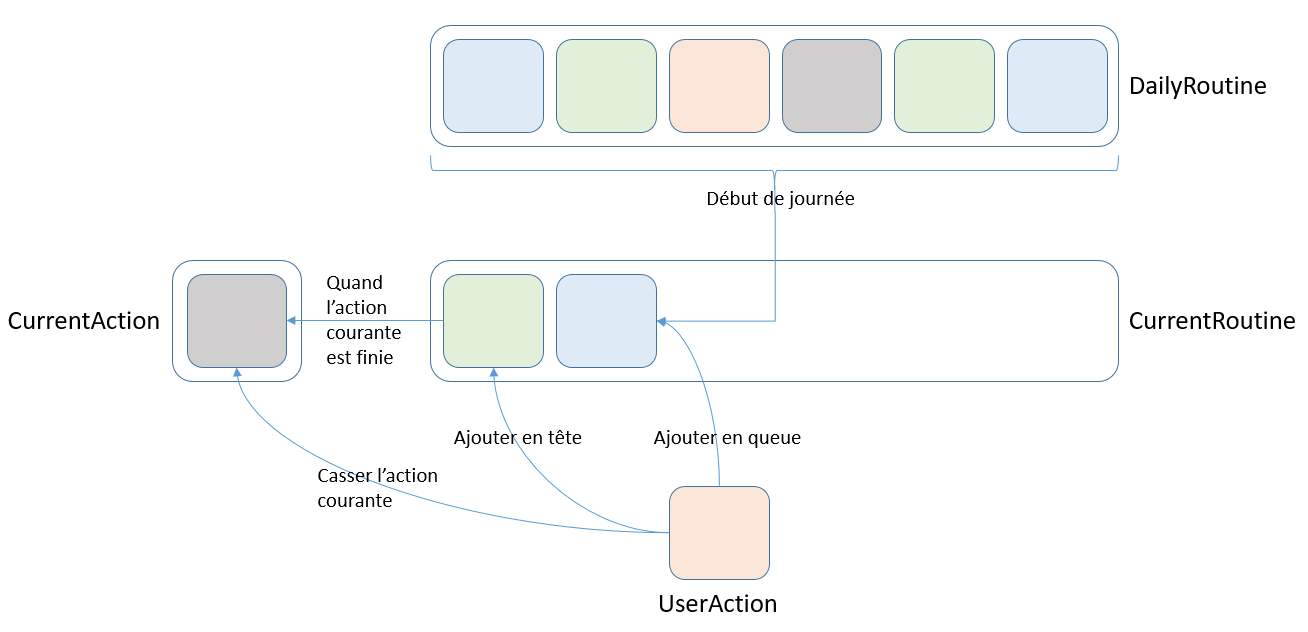
\includegraphics[width=400pt]{images/schemaRoutine.PNG}
  \caption{Fonctionnement de la routine} \label{fig:fonctionnementRoutine}
\end{figure}

\paragraph{}
La liste d'actions communes a chaque journ�es est stock� dans la liste DailyRoutine. 
A chaque d�but de journ�e, on ajoute toutes les actions de cette liste a la de la journ�e courante, CurentRoutine. 
La currentRoutine � les m�me propri�t�s qu'une files mais avec plus de possibilit� d'ajout d'actions. 
On d�file currentRoutine et on ajoute cette action � l'action courante, currentAction. 
Cette action est ex�cut� par le personnage et lorsqu'elle est finie, on d�file � nouveau la currentRoutine. 
Enfin l'utilisateur peut soit ajouter un action en t�te ou en queue dans la currentRoutine ou il peut casser l'action courante du personnage mais cela engendra un malus d?�motion.

\subsubsection{Calcul d'itin�raire}

\subsection{L'interface homme/machine}

\paragraph{}
L'interface graphique est compos� de plusieurs �l�ments�:
\begin{itemize}
 \item L'horloge du jeu, permettant de savoir quelle est la date et l'heure dans notre ville fictive
 \item La map, ou nous pouvons voir les infrastructures, et les personnages se d�placer
 \item La liste des personnages accompagn� de l'�tat de leur barre d'�motion
\end{itemize}

\paragraph{}
Chacun de ces �l�ments sont s�par� dans diff�rentes classes qui h�ritent de la classe JPanel , ce qui permet un assemblage facile de l'interface graphique, et une permutation plus facile entre diff�rentes versions d'un m�me �l�ments.

\paragraph{}
L'interface graphique est r�alis� gr�ce � Java Swing/AWT/Java 2D .

\paragraph{}
Nous pouvons voir dans le diagramme ci dessus que l'ensemble des �l�ments graphiques sont rassembl� dans une seule classe principale, qui � pour but de les assembler correctement.

\paragraph{}
La Map et la liste des personnages sont cliquables et affiche des informations en fonction de la position du curseur au moment du clique. 
Cela peut permettre d'ouvrir un autre Panel, une autre fen�tre ou autre, contenant les informations souhait�es, en fonction des situations (Pour plus de d�tail, se reporter au manuel d'utilisation). 
Ces fonctionnalit�s ont �t� impl�ment� gr�ce � des MouseListener, qui nous permettent de r�cup�rer des informations sur le curseur ou l'�tat de la souris/trackpad lors d'�v�nements pr�d�fini, lors d'un clic de souris par exemple.
\newpage
\section{Manuel Utilisateur}
\label{sec:manuel}

\subsection{D�roulement d'une partie}
\label{sec:deroulement}

\paragraph{}Une partie commence � minuit le 1er janvier 2017.

\subsubsection{Mode Normal}
\label{sec:deroulementnormal}
\paragraph{}Au d�but d'une partie en mode normal, il est possible de choisir son niveau de difficult� entre:
\begin{itemize}
\item Niveau Easy: Un seul personage sur la map
\item Niveau Normal: Trois personnes sur la map
\item Niveau Hard: Cinq personnes sur la map
\item Niveau Pro: Quinze personnes sur la map (le maximum)
\end{itemize}

\begin{figure}[H]
	\centering
		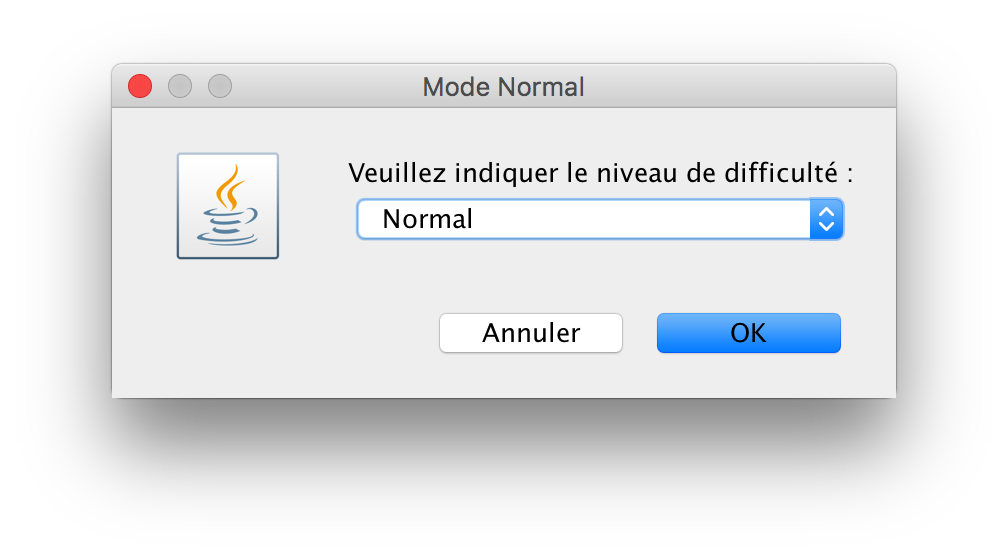
\includegraphics[width=0.5\textwidth]{images/niveau_normal.png}
		\caption{Fen�tre de selection de niveau en mode normal}
	\label{fig:nivnormal}
\end{figure}

\begin{figure}[H]
	\centering
		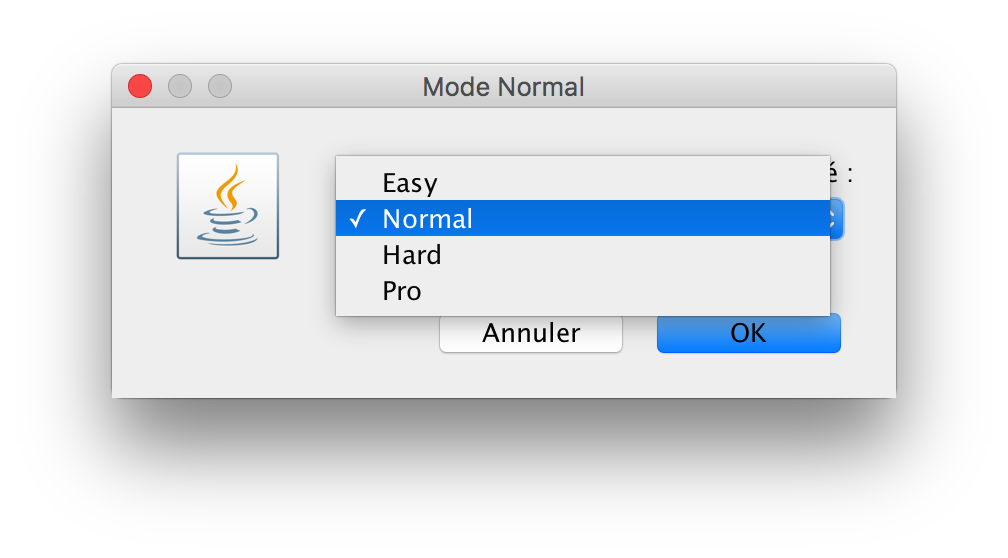
\includegraphics[width=0.5\textwidth]{images/niveausel_normal.png}
		\caption{Les differents niveau en mode normal}
	\label{fig:nivselnormal}
\end{figure}

\paragraph{}L'objectif du joueur est de faire survivre sa population le plus longtemps possible en influent sur le comportement des personnages. Un personnages meurt lorsqu'une de ces jauge (Emotion, Money, Family) arrive � 0. La partie s'arr�te quand il n'y a plus de personnages en vie.

\subsubsection{Mode Autonome}
\label{sec:deroulement_auto}
\paragraph{}En mode autonome le joueur ne peut influer sur le comportement des personnages. Le mode autonome est simulation de l'evolution d'une population dans un environnement urbain. L'utilisateur peut choisir le nombre de personnages pr�sent dans la population lors de la simulation, au d�but de la partie. Le nombre de personnages en mode autonome peut aller de 1 � 60.
\begin{figure}[H]
	\centering
		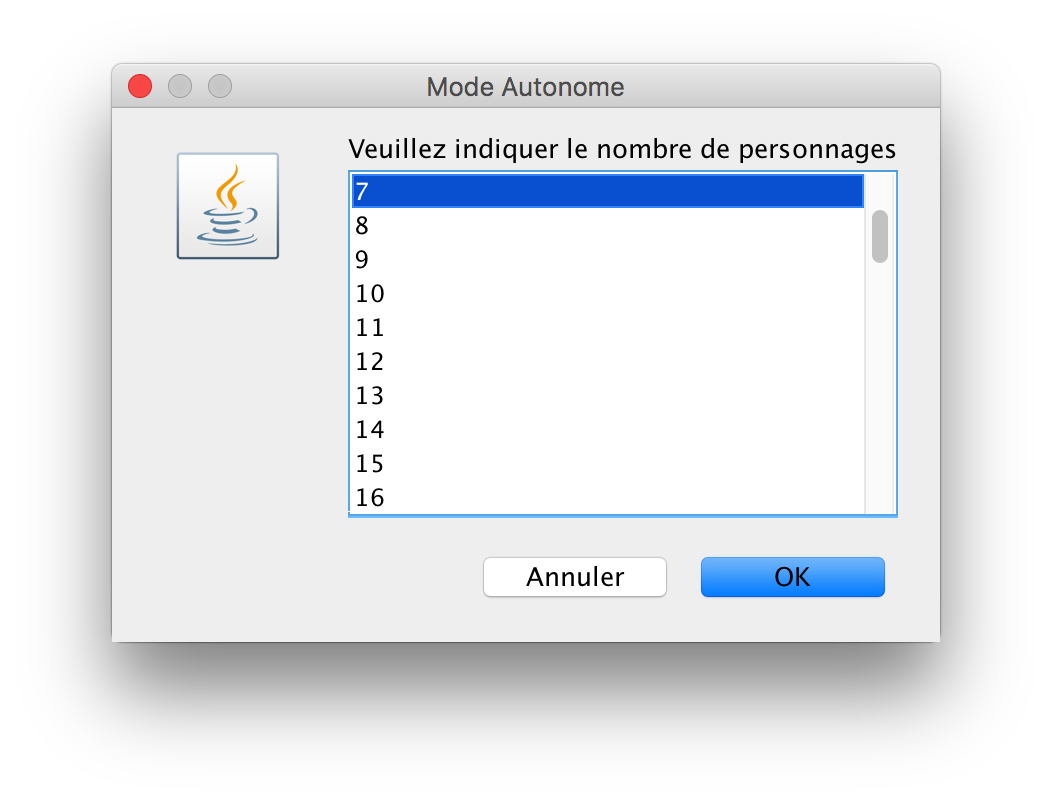
\includegraphics[width=0.5\textwidth]{images/niveau_auto.png}
		\caption{La s�lection du nombres de personnages en mode autonome}
	\label{fig:nivselauto}
\end{figure}

\paragraph{}La partie, en mode autonome, ne se fini jamais. En effet lorsqu'une des jauges d'un personnages arrive � 0, ce personnage d�m�nage et commence une nouvelle vie, jusqu'� arriver � vivre une vie stable.


\subsection{Manuel de l'IHM}
\label{sec:manIHM}

\begin{figure}[H]
	\centering
		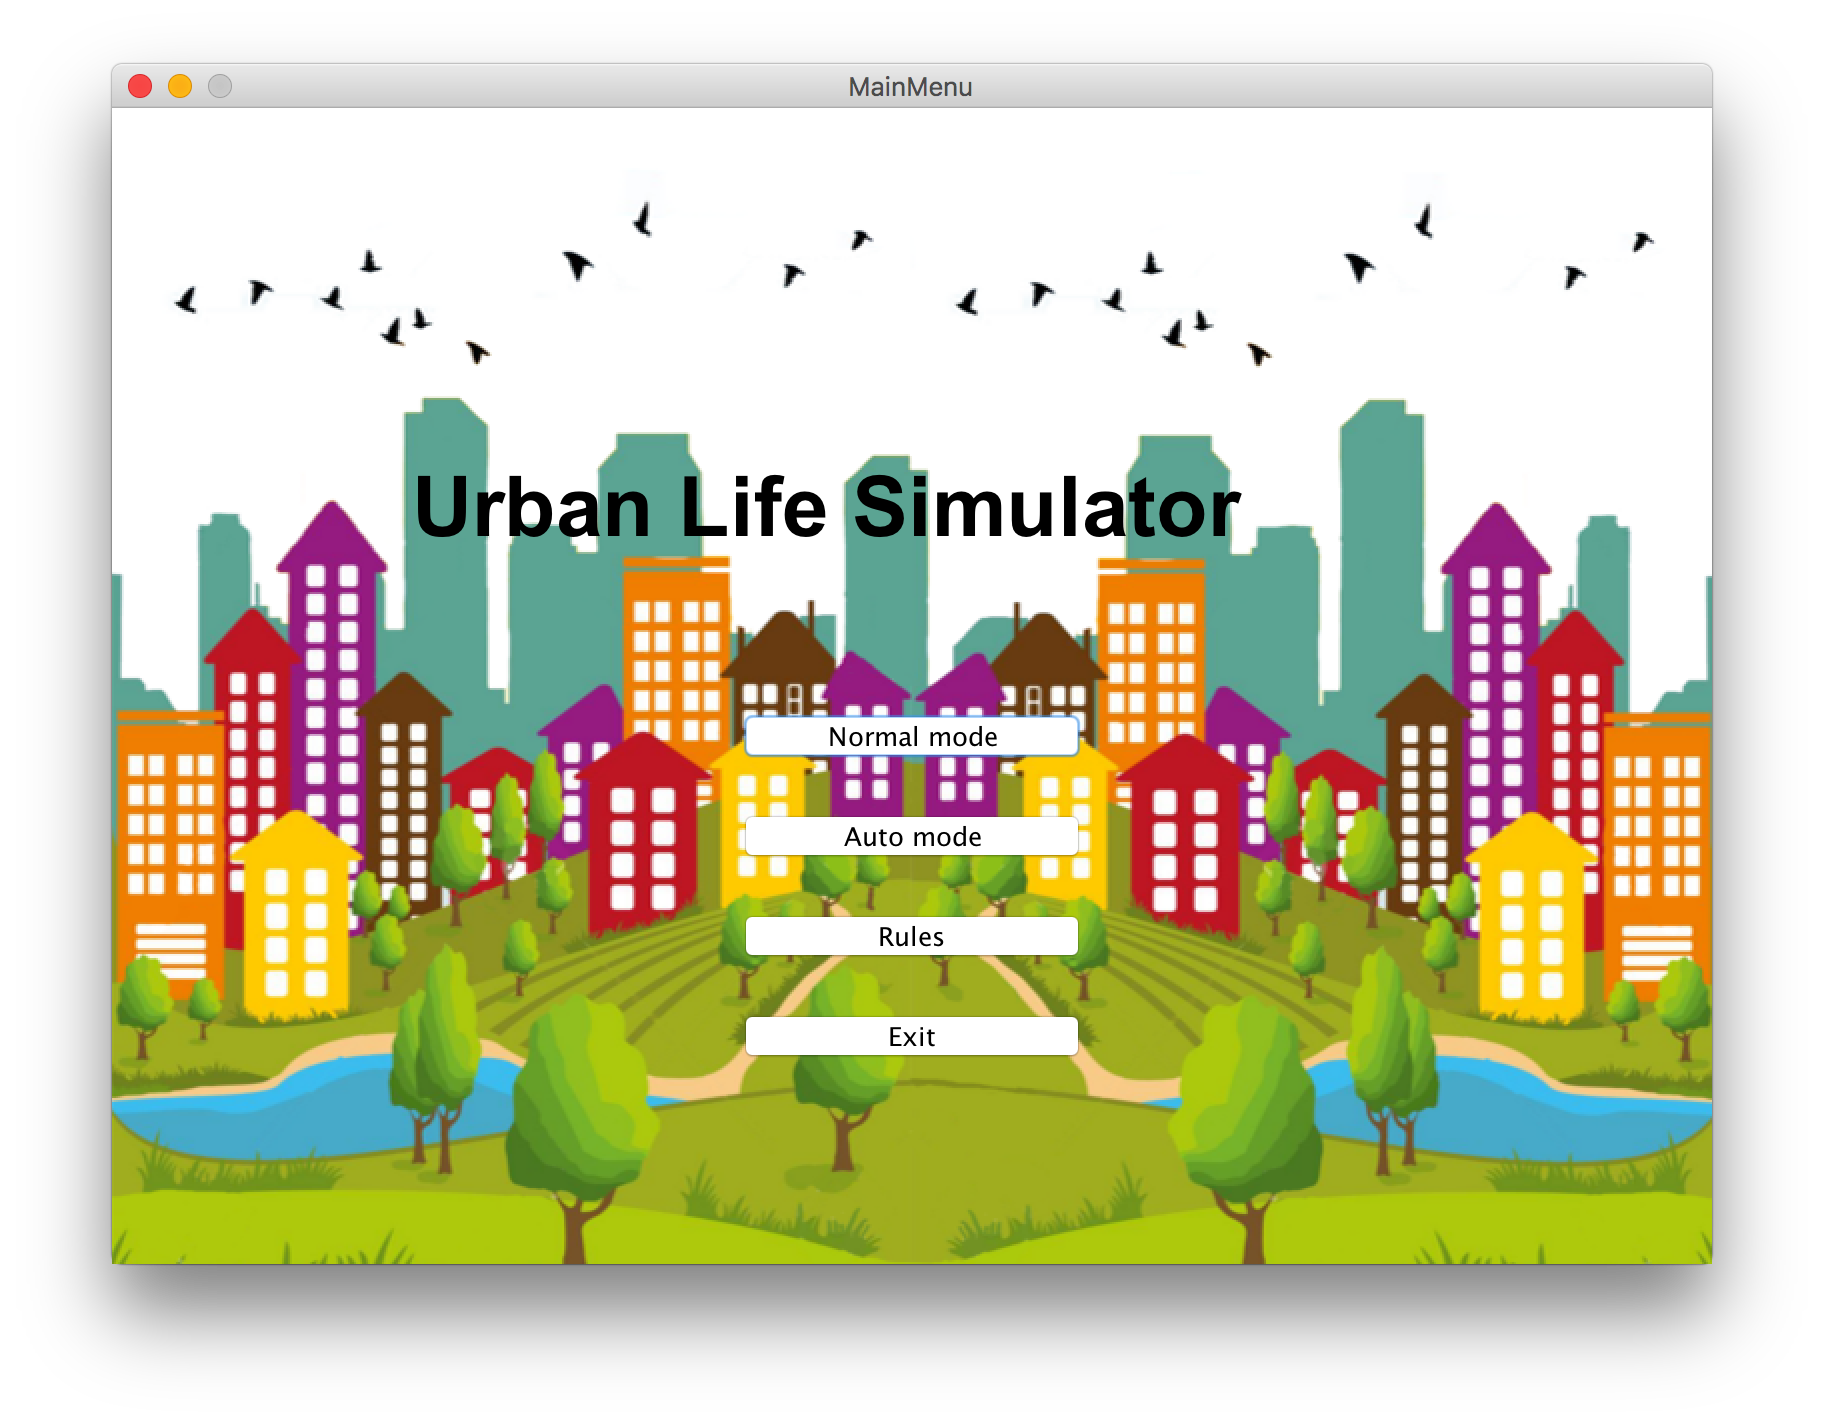
\includegraphics[width=0.75\textwidth]{images/mainmenu.png}
		\caption{Menu principal}
	\label{fig:mainmenu}
\end{figure}

\begin{figure}[H]
	\centering
		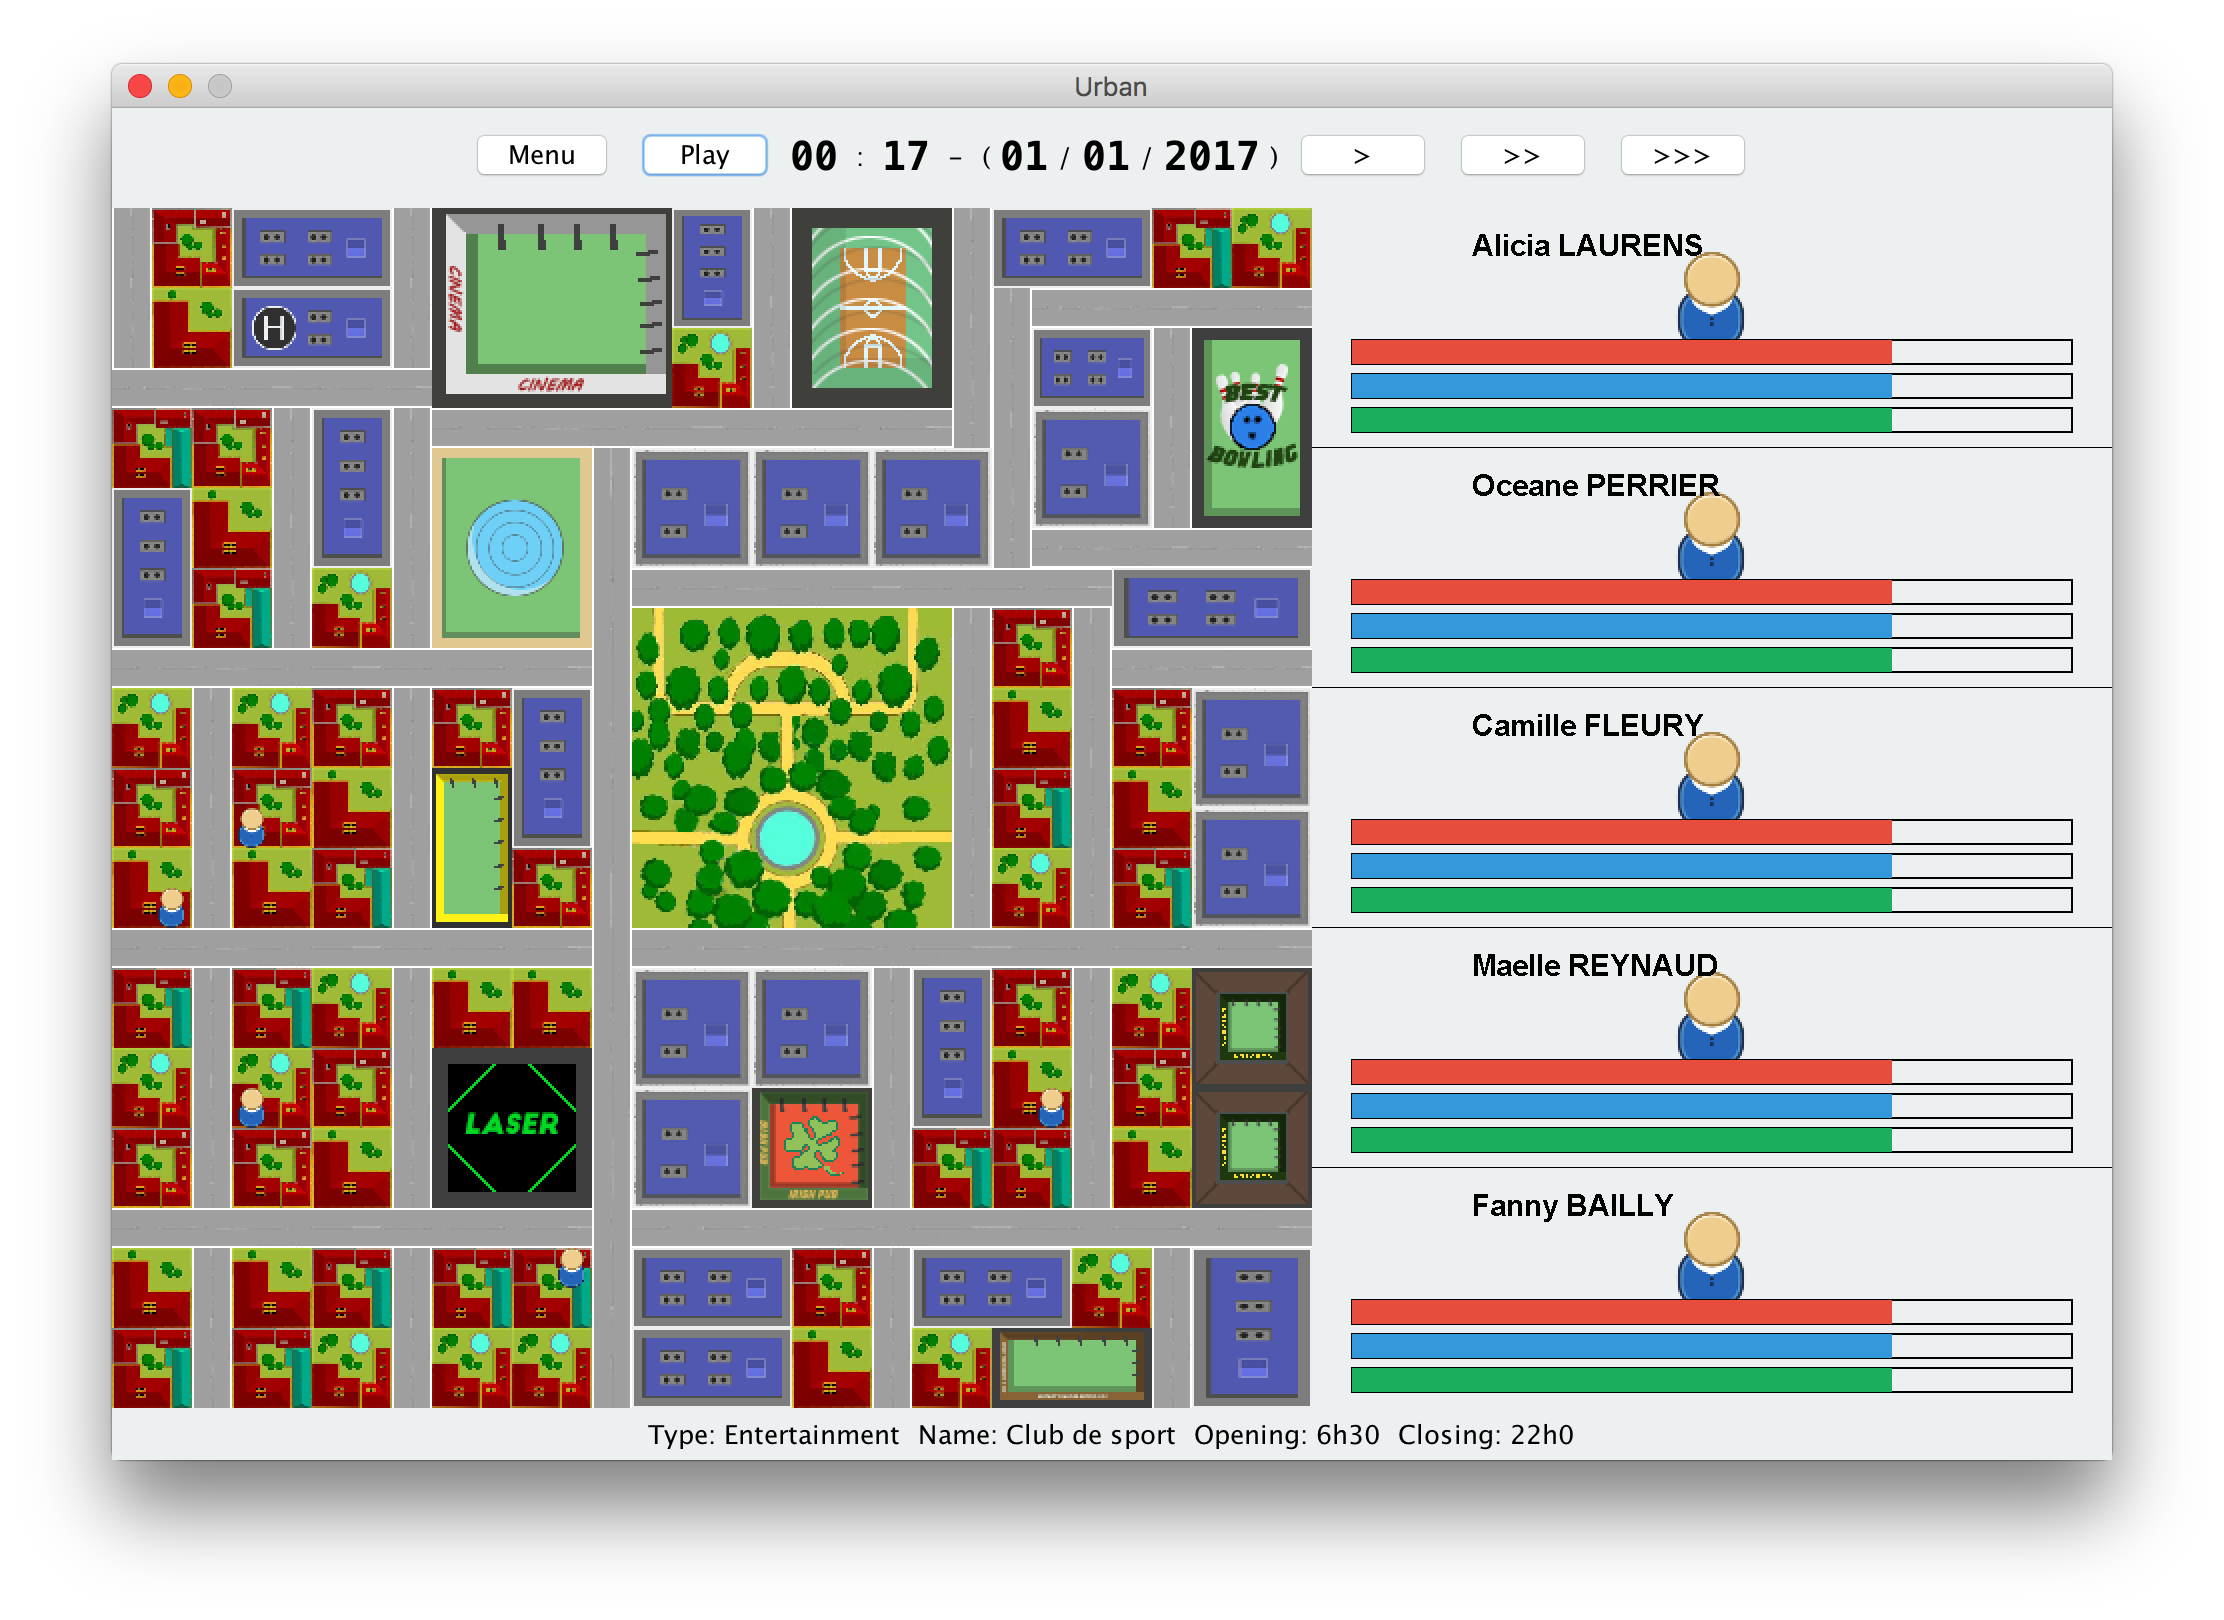
\includegraphics[width=0.75\textwidth]{images/ingame_1.png}
		\caption{IHM du jeu}
	\label{fig:ingame1}
\end{figure}


\subsubsection{Information des Infrastructures}
\label{sec:maninfrainfo}
\begin{figure}[H]
	\centering
		
\includegraphics[width=0.75\textwidth]{images/maninfrainfo.png}
		\caption{Information des infrastructures}
	\label{fig:maninfreinfo}
\end{figure}
\paragraph{}Pour afficher les informations d'une infrastructure, l'utilisateur peut double-cliquer sur n'importe qu'elle infrastructure sur la map.

\subsubsection{Information de l'Horloge}
\label{sec:manclock}
\begin{figure}[H]
	\centering
		
\includegraphics[width=0.75\textwidth]{images/manclock.png}
		\caption{Information sur l'horloge}
	\label{fig:manclock}
\end{figure}
\paragraph{}Cette partie, en plus de contenir les informations sur l'horloge rafraichie automatiquement, contient 5 boutons: (Fig.~\ref{fig:manclock})
\begin{itemize}
\item Bouton menu: permet de revenir au menu principal (Met fin � la partie)
\item Bouton Play/Pause: Permet de stopper l'horloge et de la faire reprendre
\item Bouton Speed: 3 niveau disponible permettant de r�gler la rapidit� de l'horloge
\end{itemize}

\subsubsection{La Map}
\label{sec:manmap}
\begin{figure}[H]
	\centering
		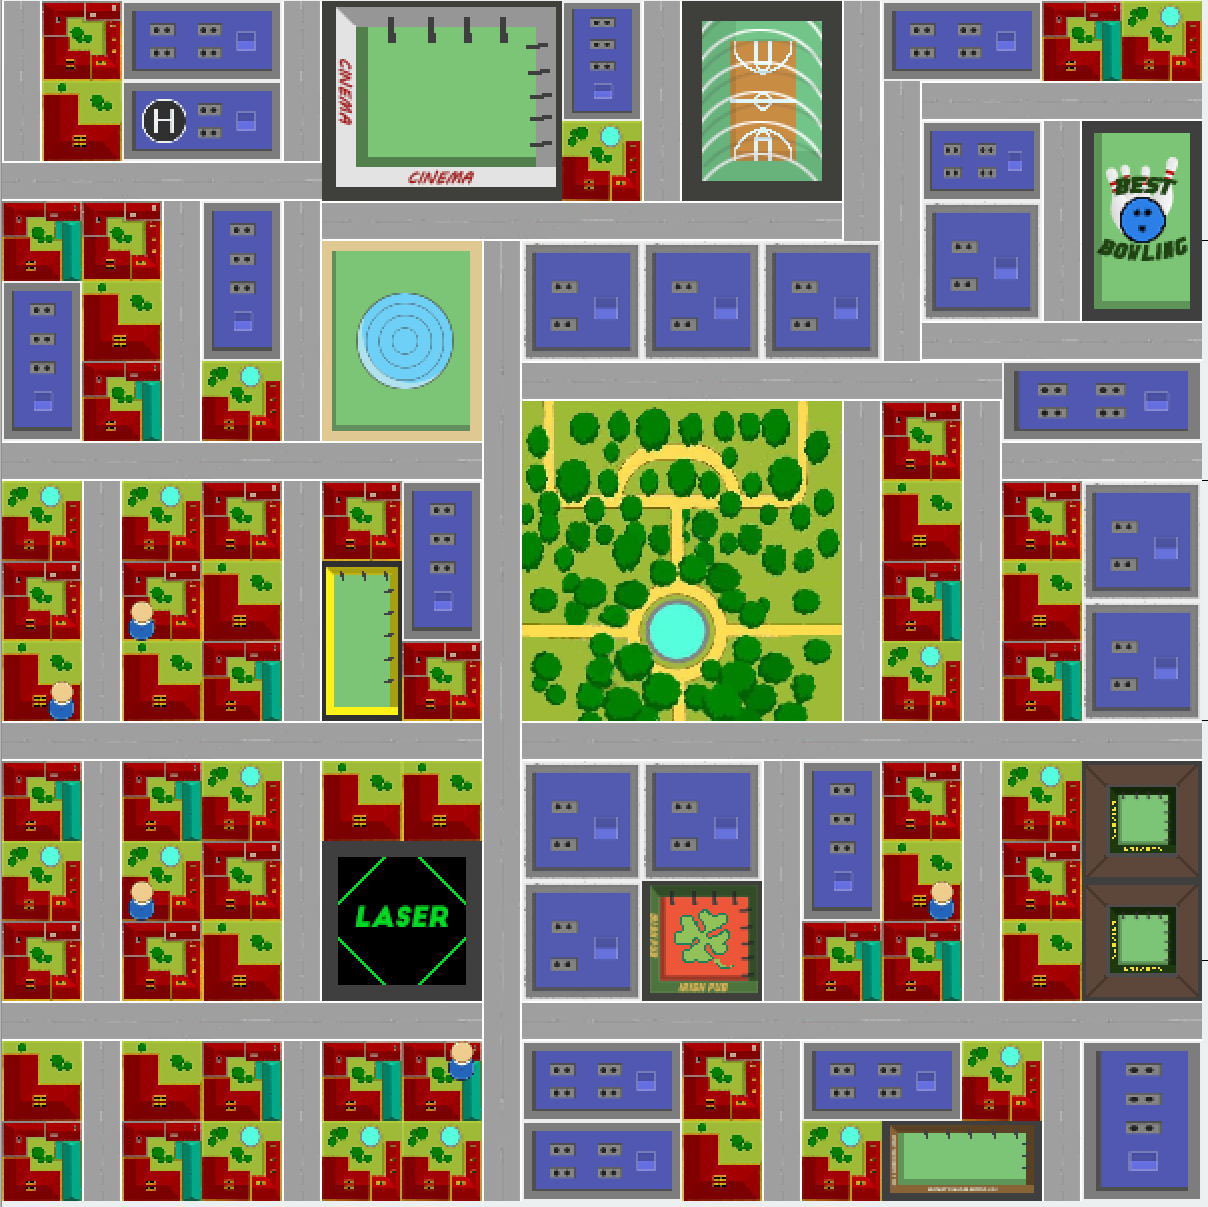
\includegraphics[width=0.5\textwidth]{images/manmap.png}
		\caption{Affichage de la Map}
	\label{fig:manmap}
\end{figure}
\paragraph{}La Map est un affichage de la situation de la population dans son environnement, � l'instant T, elle ne poss�de pas de bouton permettant de la controler.

\subsubsection{Liste des personnages}
\label{sec:manlist}
\begin{figure}[H]
	\centering
		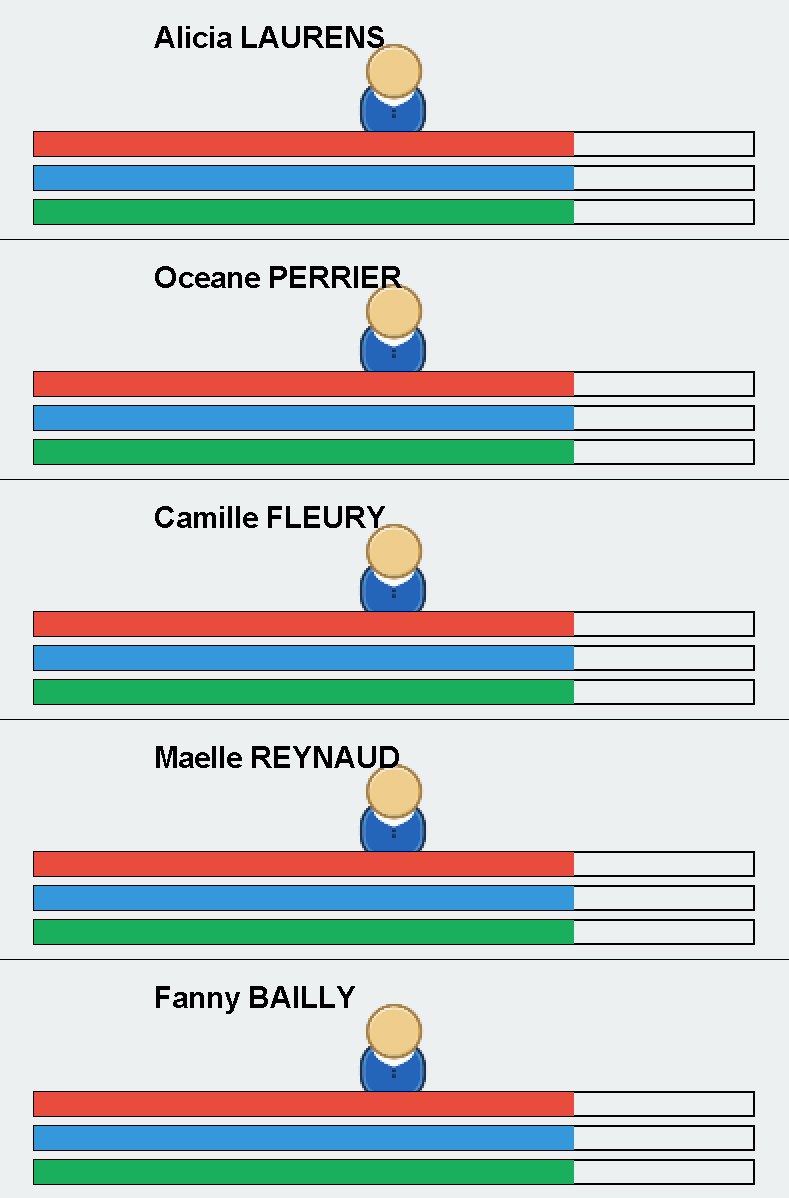
\includegraphics[width=0.3\textwidth]{images/manlist.png}
		\caption{Liste des personnages}
	\label{fig:manlist}
\end{figure}
\paragraph{}Dans cette partie de l'interface, nous pouvons voir graphiquement l'�tat de chaque personnages de la population. Toutes les informations essentiels sont directement accessible visuellement, tel que:
\begin{itemize}
\item Le nom du personnage
\item La jauge "Emotion" (en rouge)
\item La jauge "Money" (en bleu)
\item La jauge "Family" (en vert)
\end{itemize}
\begin{figure}[H]
	\centering
		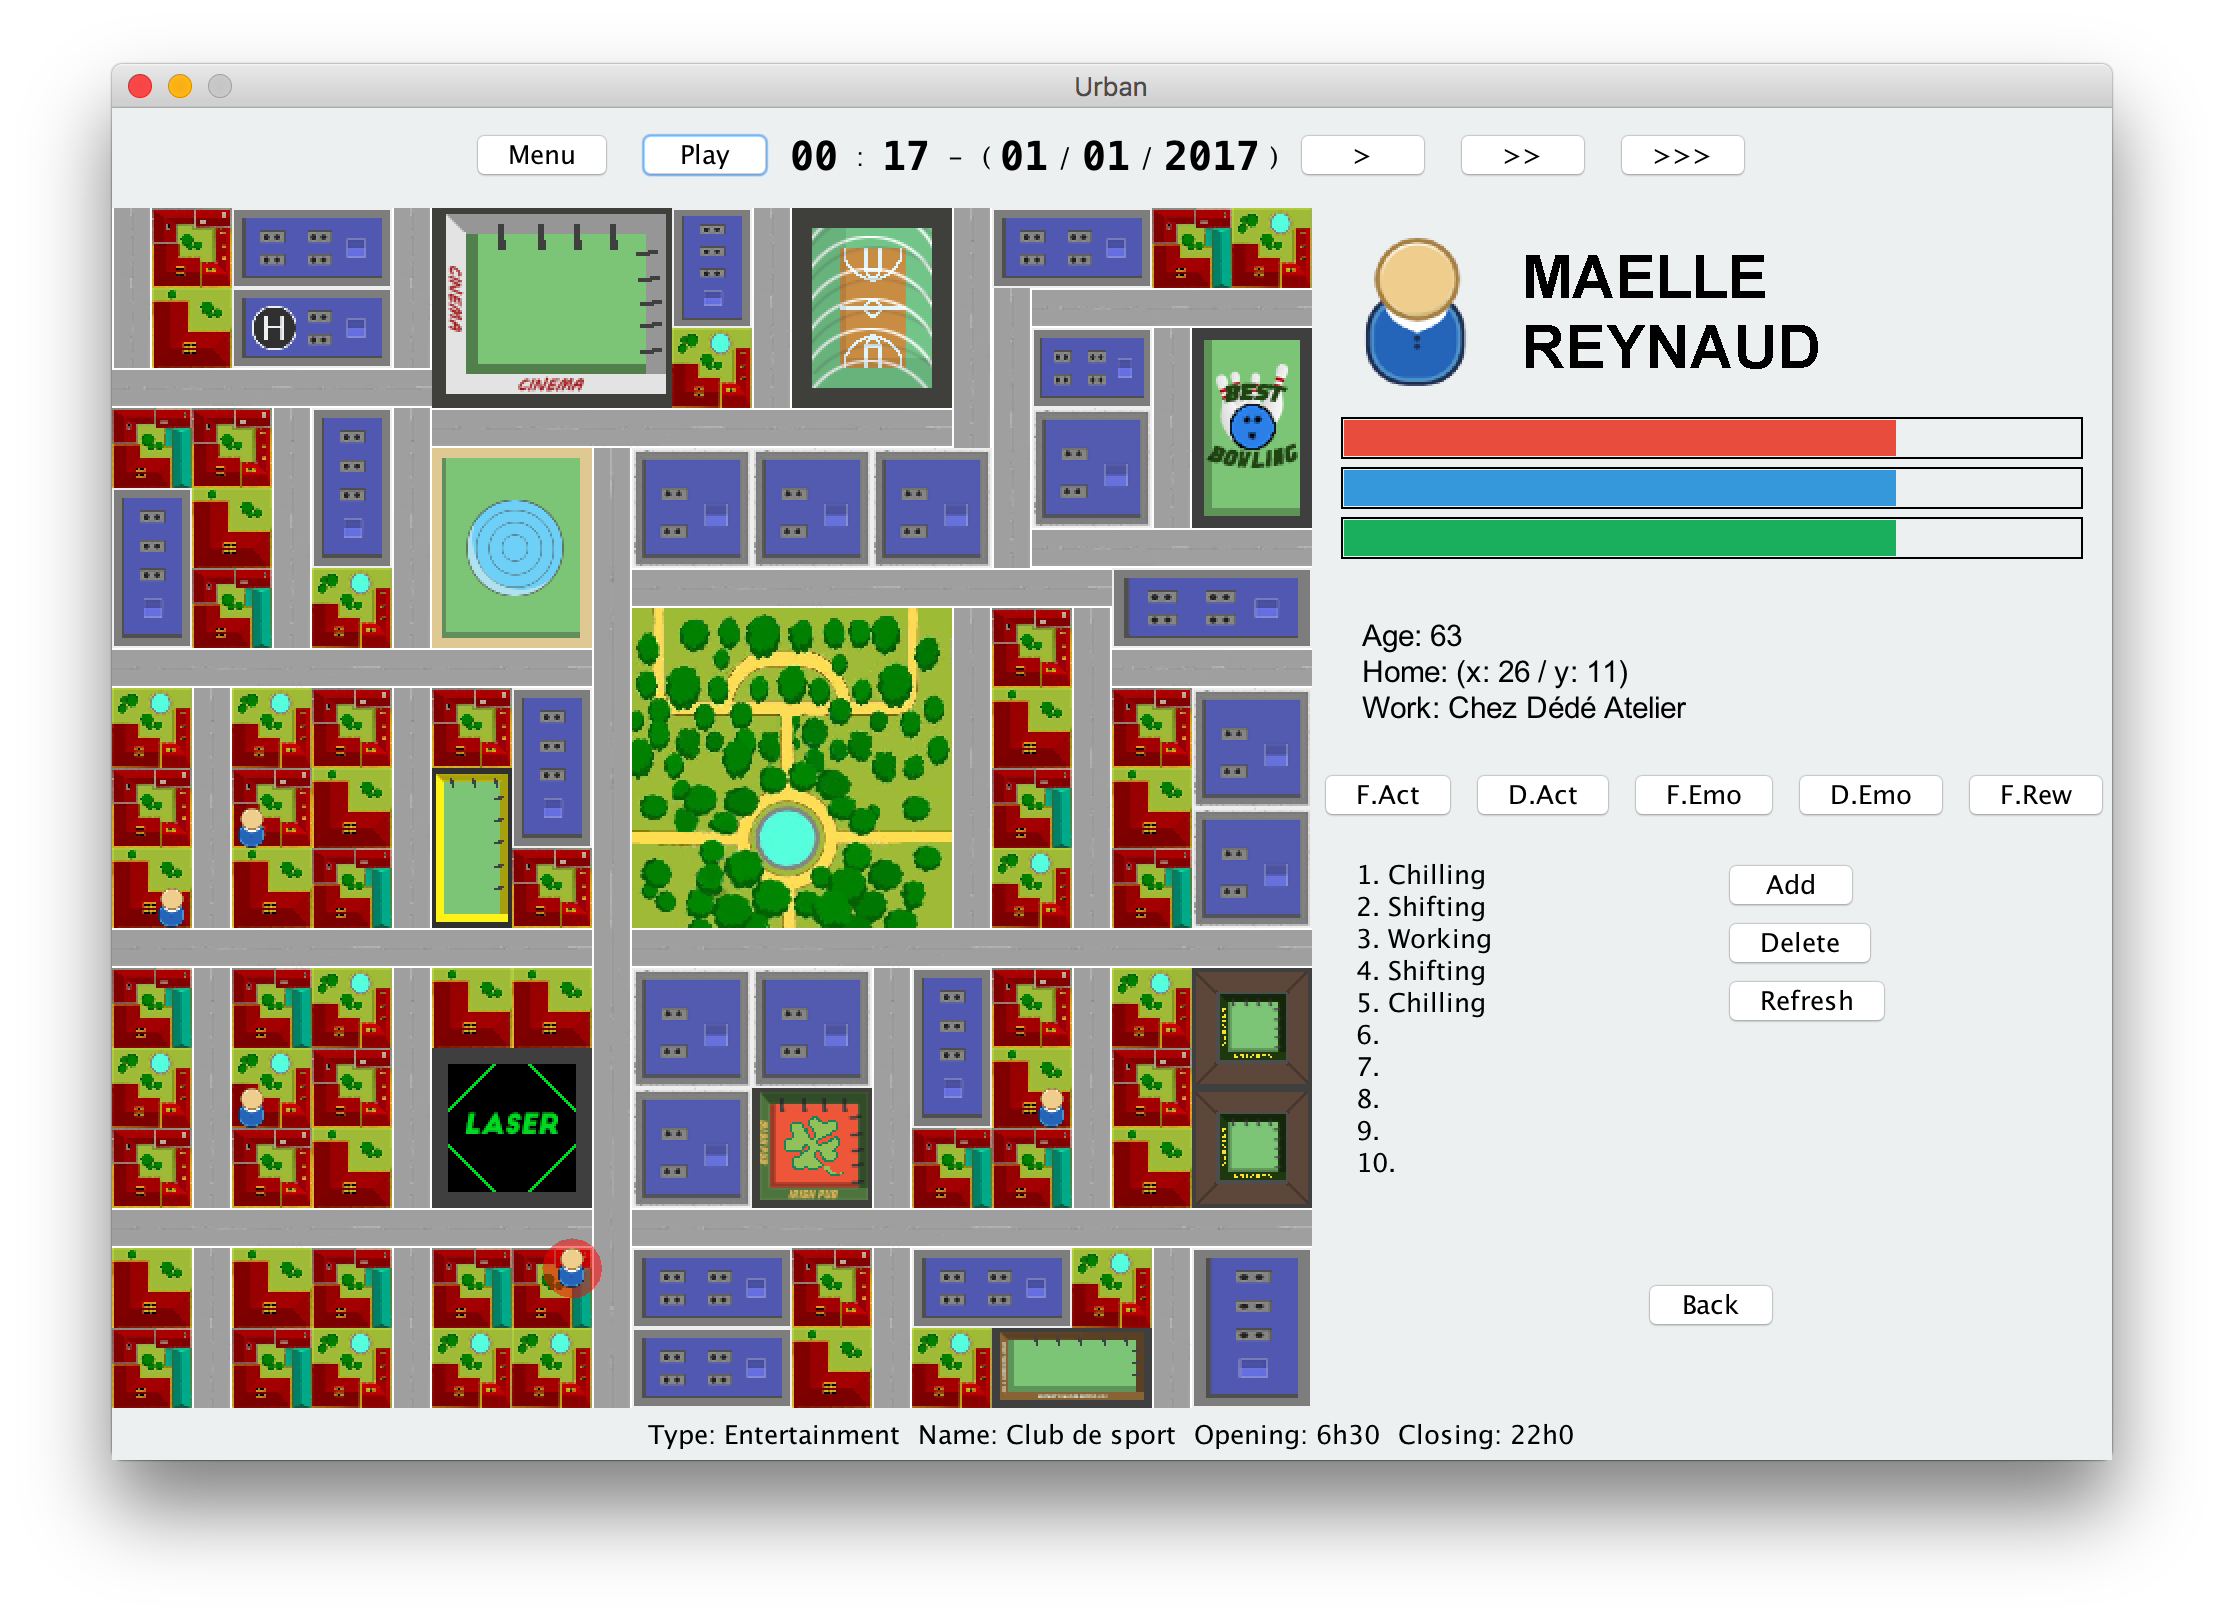
\includegraphics[width=0.75\textwidth]{images/ingame_2.png}
		\caption{Affichage de l'IHM avec les informations d�taill� sur un personnage}
	\label{fig:ingame2}
\end{figure}
\paragraph{}Afin d'acceder � plus d'options et d'informations sur un personnages, il vous suffit de cliquer sur la case d'un personnages. Vous aller ensuite arriver sur l'interface de gestion d'un personnage qui remplace la liste des personnages.
\begin{figure}[H]
	\centering
		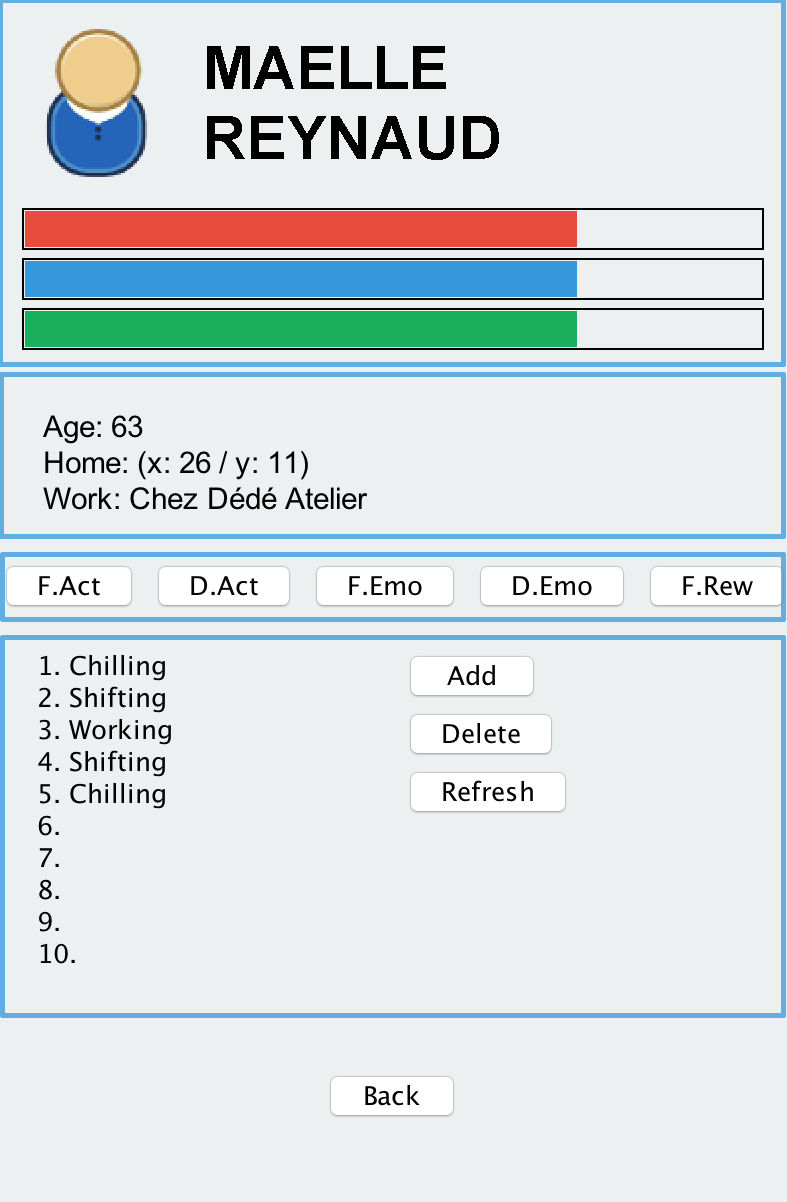
\includegraphics[width=0.25\textwidth]{images/mancharacgest.png}
		\caption{Interface de gestion d'un personnage}
	\label{fig:mancharacgest}
\end{figure}
\paragraph{}L'interface de gestion d'un personnage est divis� en 4 parties: (Fig.~\ref{fig:mancharacgest})
\begin{itemize}
\item Les informations essentiels
\item Les informations d�taill� comprenant:
\begin{itemize}
\item L'age du personnages
\item Sa maison
\item Son lieu de travail
\end{itemize}
\item Les boutons pour acc�der aux statistiques
\item La gestion de la routine comprenant:
\begin{itemize}
\item La liste des actions dans la routine courante du personnage
\item Un bouton pour ajouter une action dans la routine
\item Un bouton pour supprimer une action dans la routine du personnage
\item Un bouton pour rafraichir la liste des actions dans la routine courante du personnage
\end{itemize}
\item Un bouton pour revenir � la liste des personnages
\end{itemize}
\begin{figure}[H]
	\centering
		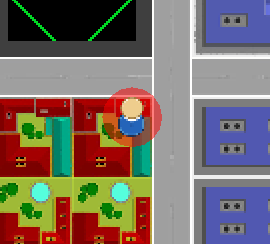
\includegraphics[]{images/manredcircle.png}
		\caption{Le personnage "Maelle Reynaud" d�marqu� par un cercle rouge}
	\label{fig:manredcircle}
\end{figure}
\paragraph{}Lorsqu'un personnage est s�l�ctionner dans la liste et que l'interface de gestion du personnage est activ�, le personnage est d�marqu� sur la map pour pouvoir le suivre plus facilement. En effet, dans ce cas l�, un cercle rouge est pr�sent derri�re l'image representant le joueur, pour le rep�rer plus facilement.(Fig.~\ref{fig:manredcircle})

\subsubsection{Les statistiques}
\label{sec:manstat}
\paragraph{}L'utilisateur peut acc�der � 5 graphiques (g�n�raient gr�ce � la bilbioth�que JFreeChart) repr�sentant l'�volution du personnages s�l�ctionn�, au cours du temps, en cliquant sur l'un des 5 boutons pr�sent dans l'interface de gestion de personnages. Parmi les graphiques nous pouvons trouver, par ordre d'apparition:
\begin{itemize}
\item La r�partition des actions du personnage
\item La r�partition des actions du personnage sur la journ�e en cours et celle de la veille
\item L'�volution des jauge Emotion, Money et Family du personnages
\item L'�volution des jauge Emotion, Money et Family du personnages sur la journ�e en cours et celle de la veille
\item La r�partition des recompense (r�compense positive, n�gative et nulle) du personnage
\end{itemize}

\subsubsection{La routine}
\label{sec:manroutine}
\subsubsubsection{Ajout d'action dans la routine}
\label{sec:manaddaction}
\begin{figure}[H]
	\centering
		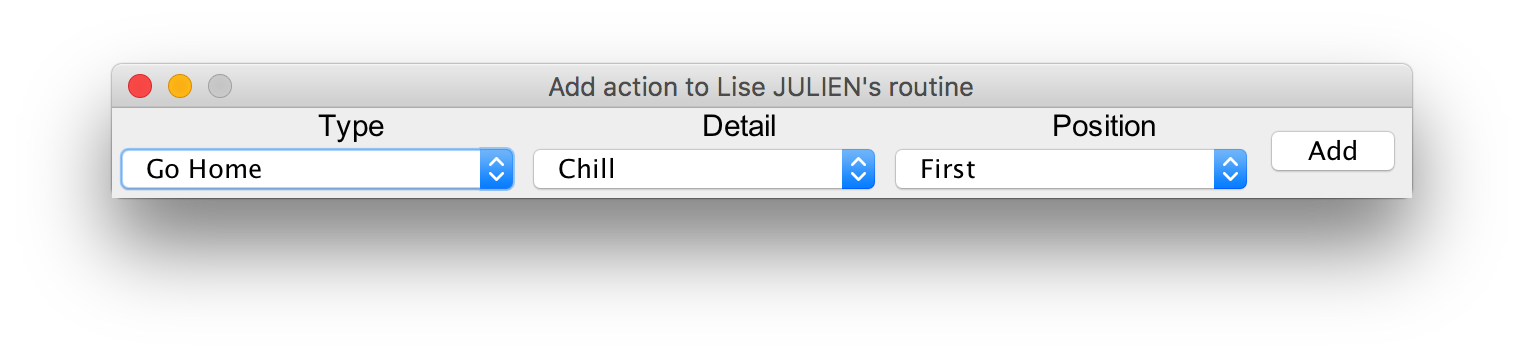
\includegraphics[width=0.75\textwidth]{images/manaddaction.png}
		\caption{Fen�tre d'ajout d'action d'un personnage}
	\label{fig:manaddaction}
\end{figure}
\paragraph{}Pour acc�der � l'interface d'ajout d'action dans la routine, l'utilisateur doit cliquer sur le bouton "Add" pr�sent dans l'interface de gestion d'un personnage.
\begin{figure}[H]
	\centering
		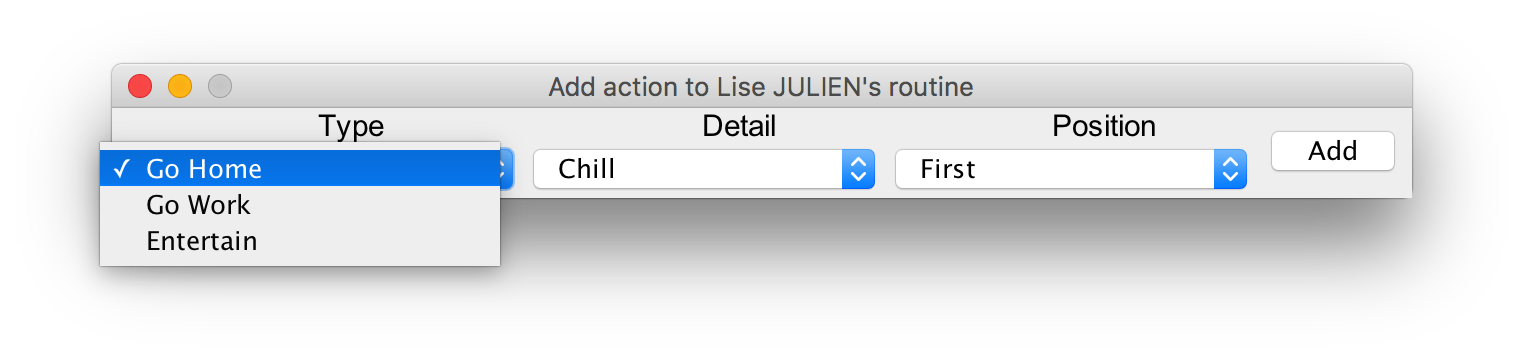
\includegraphics[width=0.75\textwidth]{images/manactionchoice.png}
		\caption{Choix d'action disponible}
	\label{fig:manactionchoice}
\end{figure}
\paragraph{}L'utilisateur � le choix entre 3 type d'actions:(Fig.~\ref{fig:manactionchoice})
\begin{itemize}
\item Go Home
\item Go Work
\item Entertain
\end{itemize}

\begin{figure}[H]
	\centering
		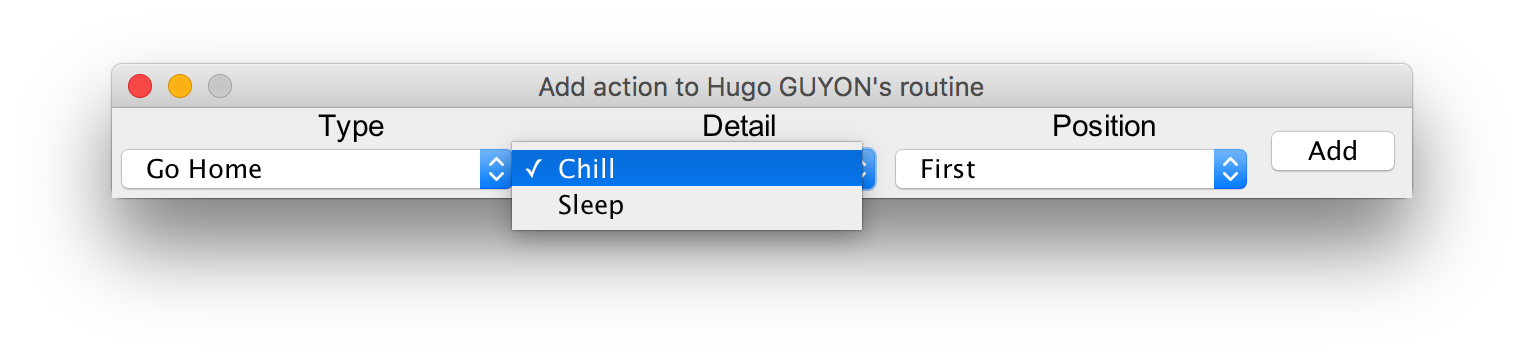
\includegraphics[width=0.75\textwidth]{images/mandetailhome.png}
		\caption{Choix de detail lors du choix d'une action de type Go Home}
	\label{fig:mandetailhome}
\end{figure}
\paragraph{}Lorsque l'utilisateur choisit une action de type "Go Home", il peut sp�cifier si le personnage doit dormir, ou juste se reposer.(Fig.~\ref{fig:mandetailhome})

\begin{figure}[H]
	\centering
		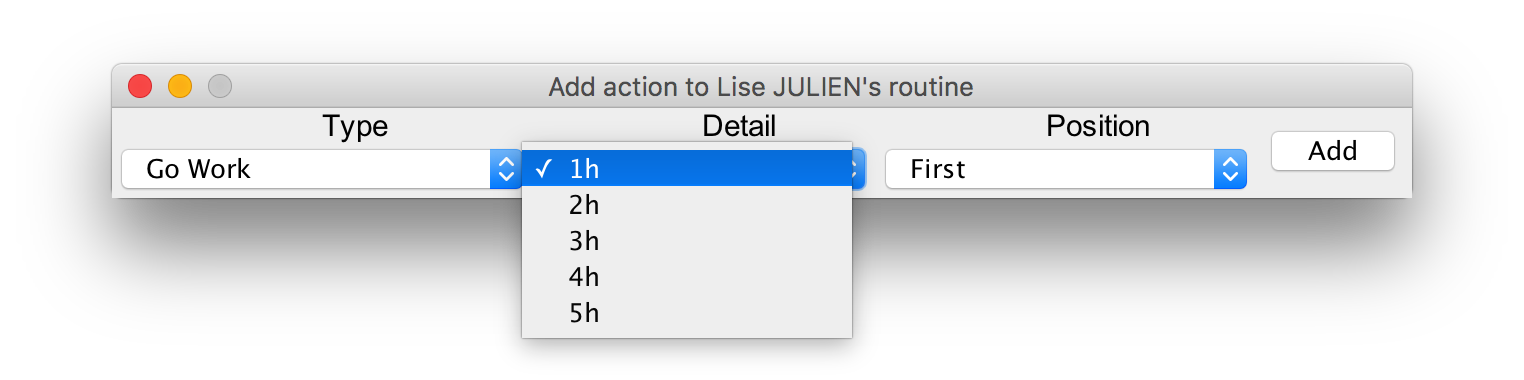
\includegraphics[width=0.75\textwidth]{images/mandetailwork.png}
		\caption{Choix de detail lors du choix d'une action de type Go Work}
	\label{fig:mandetailwork}
\end{figure}
\paragraph{}Lorsque l'utilisateur choisit une action de type "Go Work", il peut sp�cifier combien de temps le personnages doit travailler.(Fig.~\ref{fig:mandetailwork})

\begin{figure}[H]
	\centering
		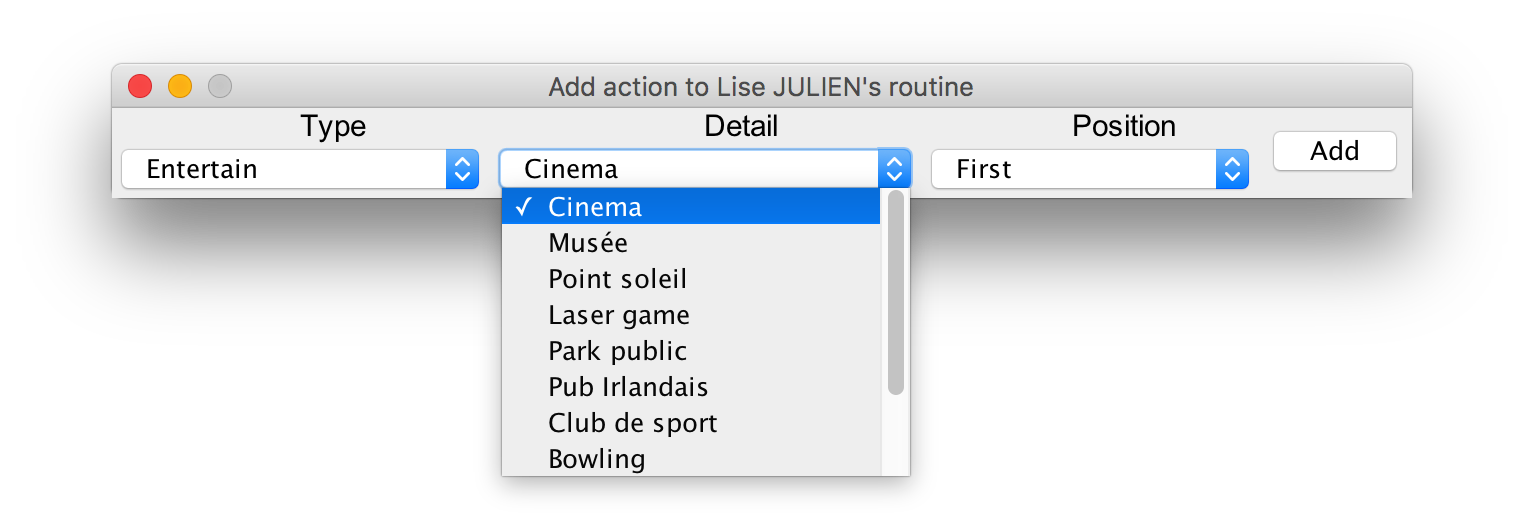
\includegraphics[width=0.75\textwidth]{images/mandetailenter.png}
		\caption{Choix de detail lors du choix d'une action de type Entertain}
	\label{fig:mandetailwork}
\end{figure}
\paragraph{}Lorsque l'utilisateur choisit une action de type "Entertain", il peut sp�cifier o� le personnages ira se divertir.(Fig.~\ref{fig:mandetailenter})

\begin{figure}[H]
	\centering
		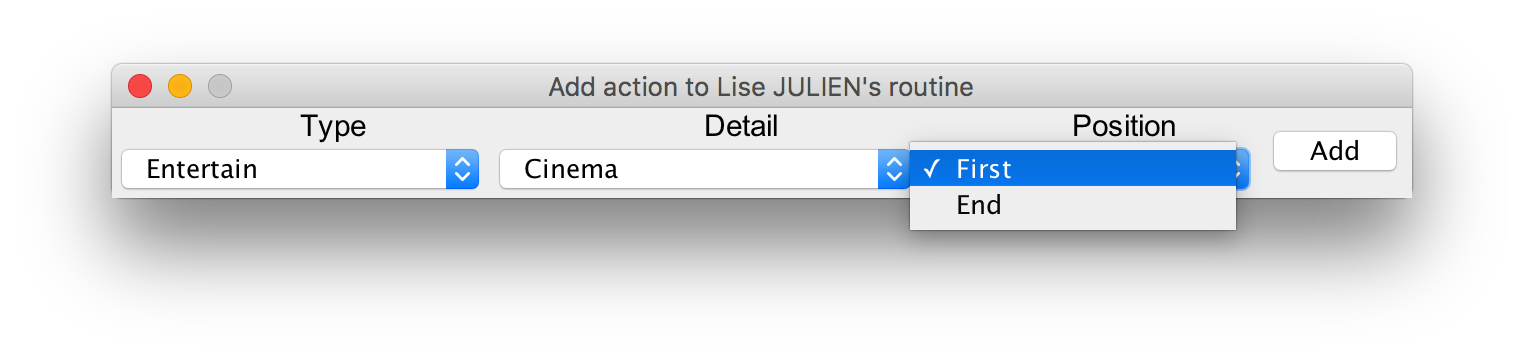
\includegraphics[width=0.75\textwidth]{images/manpositionchoice.png}
		\caption{Choix de la position de l'ajout de l'action}
	\label{fig:manpositionchoice}
\end{figure}
\paragraph{}L'utilisateur � le choix, lors de l'ajout d'une action, de la position de l'action dans la routine courante (En premier ou en dernier)(Fig.~\ref{fig:manpositionchoice})

\paragraph{}Pour valider l'ajout, l'utilisateur doit appuyer sur le bouton "Add". Lors de l'ajout d'une action, les actions de d�placement sont automatiquement pris en compte.

\subsubsubsection{Suppression d'action dans la routine}
\label{sec:mandeleteaction}
\begin{figure}[H]
	\centering
		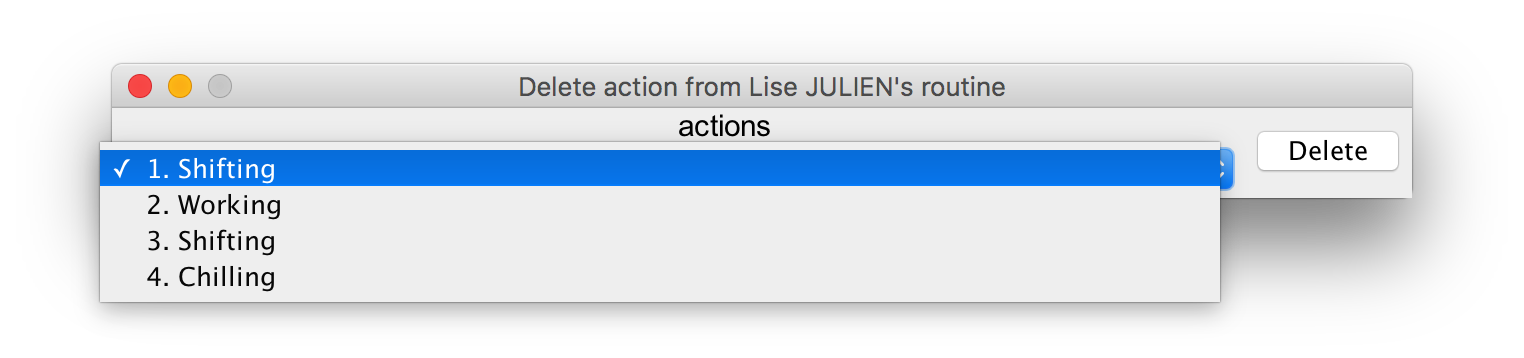
\includegraphics[width=0.75\textwidth]{images/mandelete.png}
		\caption{Fen�tre de supression d'action d'un personnage}
	\label{fig:mandelete}
\end{figure}
\paragraph{}Pour acc�der � l'interface de suppression d'action dans la routine, l'utilisateur doit cliquer sur le bouton "Delete" pr�sent dans l'interface de gestion d'un personnage.
\paragraph{}L'interface de suppression d'action est compos� de la liste d'action dans la routine courante du personnage s�lectionn�, par ordre d'execution, ainsi l'action "1" est la prochaine � �tre �xecut�. L'utilisateur peut donc choisir pr�cisement quelle action il souhaite supprimer dans la routine du personnage.(Fig.~\ref{fig:mandelete}) Pour valider la suppression l'utilisateur doit appuyer sur le bouton "Delete".

\subsection{Apr�s la partie}
\label{sec:aftergame}
\paragraph{}Une fois la partie termin� (en mode normale), un score de l'utilisateur est calculer, et le programme propose � l'utilisateur d'enregistrer son score et de consulter le classement des meilleurs joueurs � Urban Life Simulator. Son score n'apparait dans le classement que si il fait partie des 10 meilleurs joueurs dans son niveau de difficult�.
\begin{figure}[H]
	\centering
		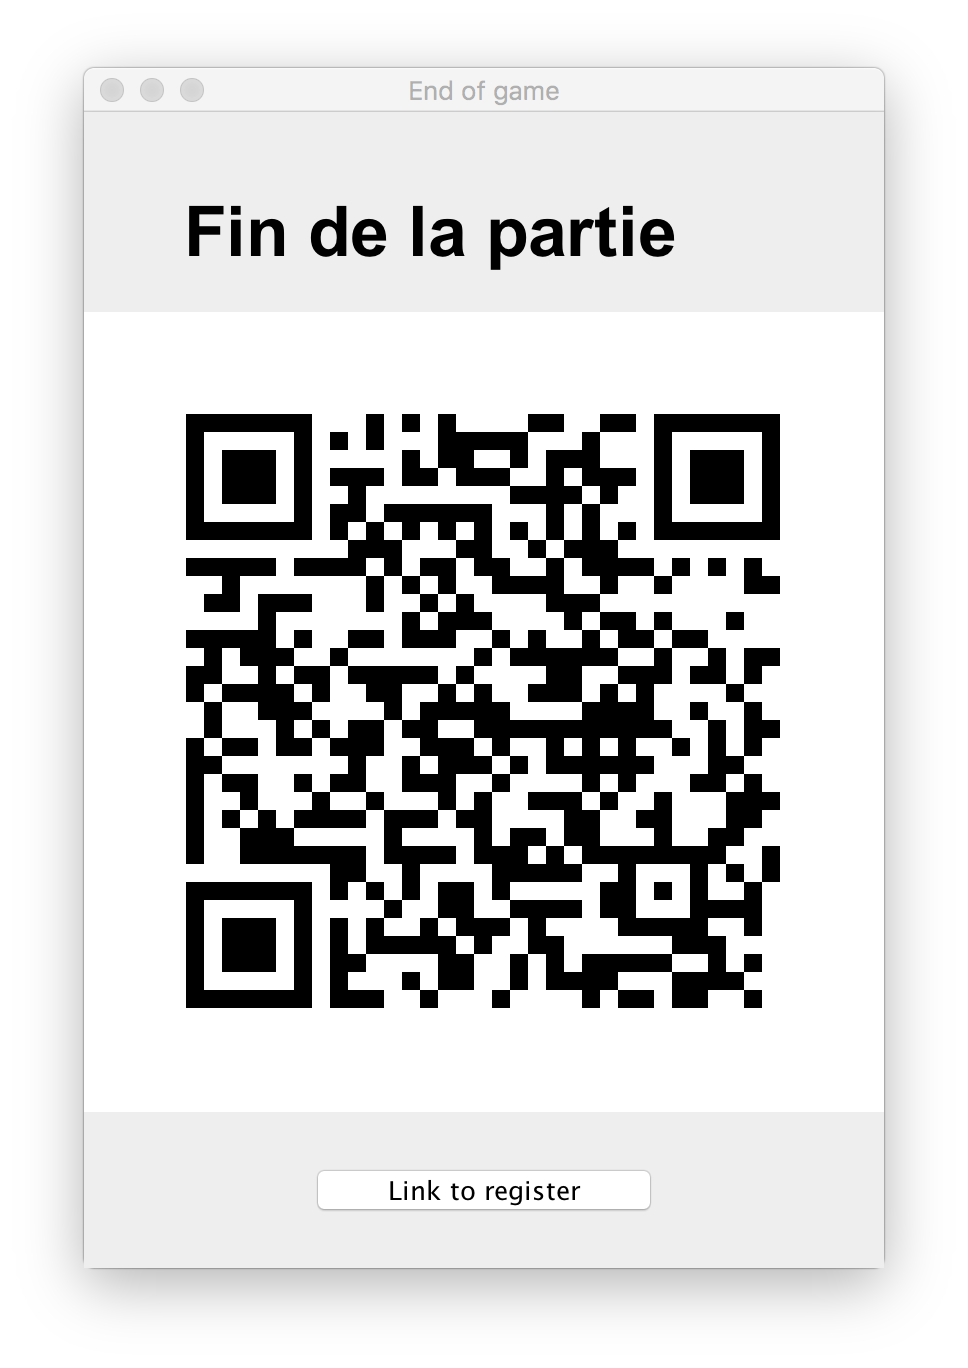
\includegraphics[width=0.25\textwidth]{images/manqrcode.png}
		\caption{Fen�tre de fin de partie avec un exemple de QR Code}
	\label{fig:manqrcode}
\end{figure}
\paragraph{}Pour enregistrer son score l'utilisateur peut scanner le QR Code unique que le jeu lui a g�n�r� (Il peut aussi directement cliquer sur le bouton en dessous du QR Code si il ne poss�de pas de lecteur de QR Code).(Fig.~\ref{fig:manqrcode}) Ce QR Code le redirige directement vers la plateforme de Leaderboard en ligne.
\begin{figure}[H]
	\centering
		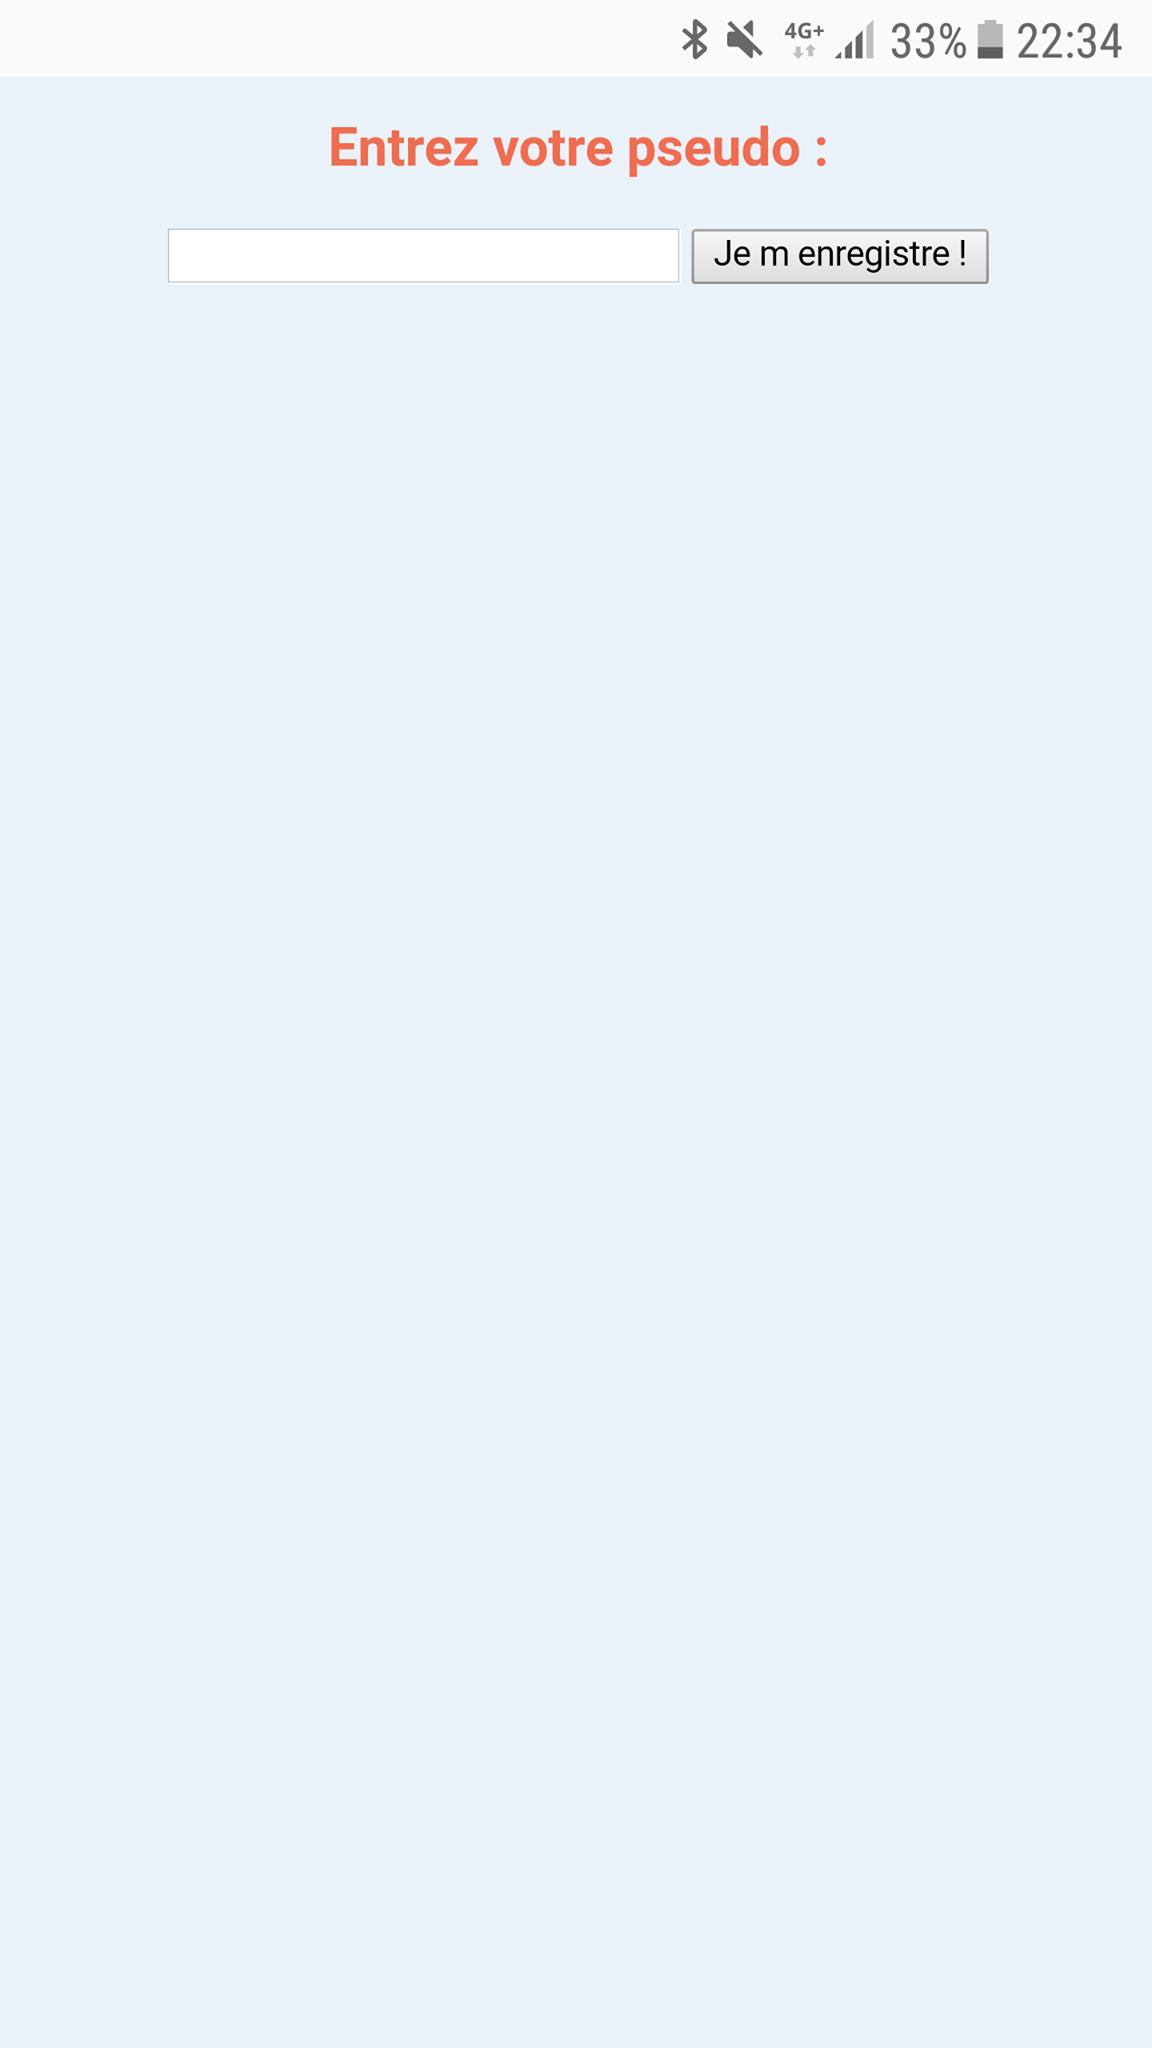
\includegraphics[width=0.25\textwidth]{images/manregscore.png}
		\caption{Fen�tre d'enregistrement du score}
	\label{fig:manregscore}
\end{figure}
\paragraph{}La page d'enregistrement est compos� d'un champ pour entrer son pseudonyme et d'un bouton pour valider.(Fig.~\ref{fig:manregscore}) Pour l'exemple nous allons mettre "Projet Urbain" comme pseudonyme. Une fois valider le site web enregistre le score dans le classement correspondant au niveau de difficult� auquel l'utilisateur a jou�, et redirige automatiquement vers la page du classement.
\begin{figure}[H]
	\centering
		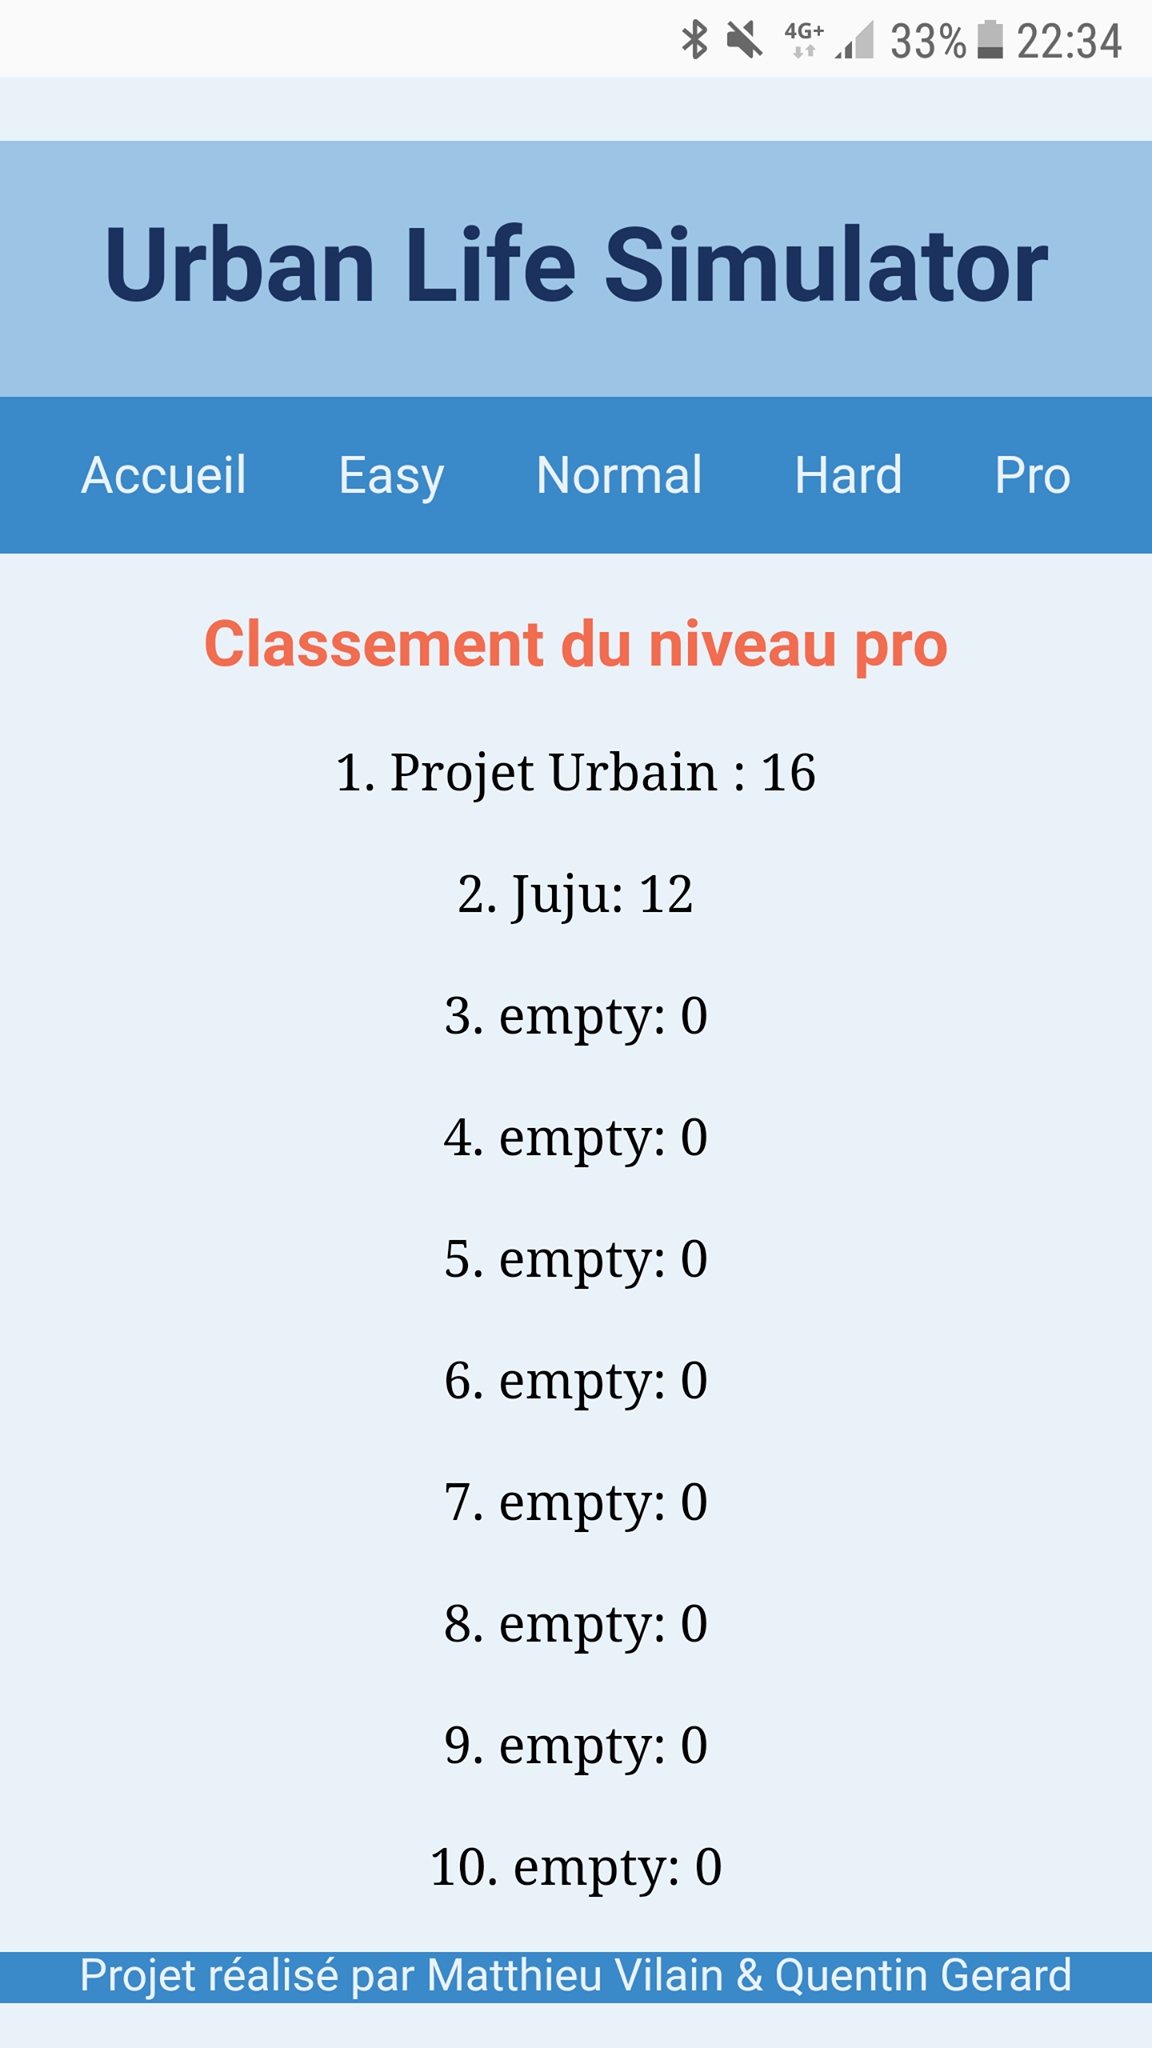
\includegraphics[width=0.25\textwidth]{images/manleader.png}
		\caption{Classement du niveau Pro}
	\label{fig:manleader}
\end{figure}
\paragraph{}Sur cette page (Fig.~\ref{fig:manleader}) l'utilisateur peut se compar� � d'autres personnes ayant jou� au jeu sur le m�me niveau de difficult� que le sien. Nous pouvons voir que lors de la partie notre joueur "Projet Urbain", a fait un score de 16 en niveau "Pro", et est donc le premier du classement au moment o� il a jou�.
\newpage
\section{D�roulement du projet}
\label{sec:deroulement}

\noindent Dans cette section, nous d�crivons comment la r�alisation du projet s'est d�roul�e au sein de l'�quipe de projet. La r�partition des t�ches, la synchronisation du travail et l'utilisation du temps seront abord�es. 

\subsection{R�partition des t�ches}

\begin{table}[H]
\centering
\begin{tabular} {|p{5cm}|p{5cm}}
\hline
\huge{Matthieu Vilain} & \huge{Quentin Gerard} \\
\hline
\multicolumn{2}{|c|}{Reflexion autour du sujet} \\
\hline
Classes de donn�es\newline partie population & Classes de don�es\newline partie ville \\
\hline
Moteur\newline Mode normal/Autonome & IHM \\
\hline
Tests unitaires & Logging \\
\hline 
Prototypage algorithmes & Cr�ation du site \\
\hline
QRCode g�neration de l'URL & fonctions PHP \\
\hline
\multicolumn{2}{|c|}{Rapport} \\
\hline
\multicolumn{2}{|c|}{Pr�sentation} \\

\end{tabular}
\caption{R�partition des t�ches}
\label{tab:document}
\end{table}


\subsection{Synchronisation du travail}

\paragraph{}
Pour la synchronisation du travail nous avons utilis� l'outil de versionnage Git coupl� � la plate-forme GitHub.
\paragraph{}
Nous avons voulu l'utiliser comme il peut �tre utilis� en entreprise : avec un environnement de production, un environnement de test et un environnement client (o� le produit est dans une version fonctionnelle).
Pour cela nous avons utilis� le syst�me de branche de Git selon le sch�ma suivant : 

\begin{figure}[H]
\centering
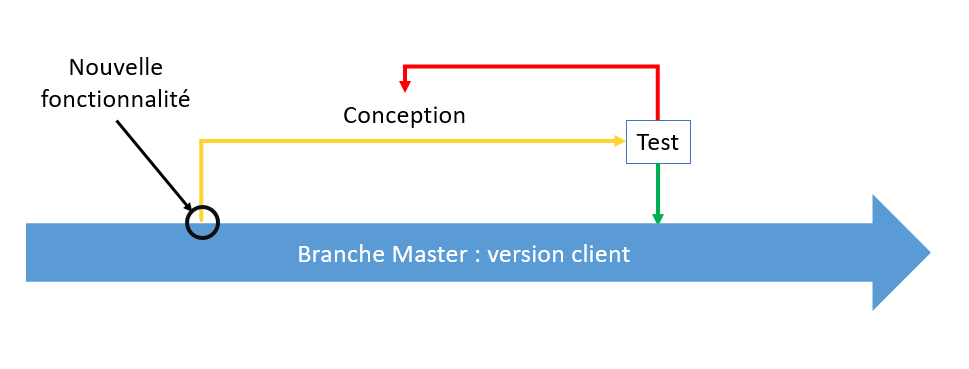
\includegraphics[width=1.0\textwidth]{images/git.PNG}
\caption{Utilisation de Git}
\label{fig:modele}
\end{figure}

\subsection{Utilisation du temps}

\paragraph{}
Pour la gestion du temps, nous avons rapidement d�velopp� toutes les classes de donn�es, les fonctionnalit�s principales et une IHM simplifi�e.
Cela nous a permis d'avoir rapidement une base de tests solide pour d�velopper les fonctionnalit�s plus complexes et une meilleure IHM.
Ensuite nous avons gard� un ryhtme constant pour ne pas prendre de retard.

\begin{figure}[H]
\centering
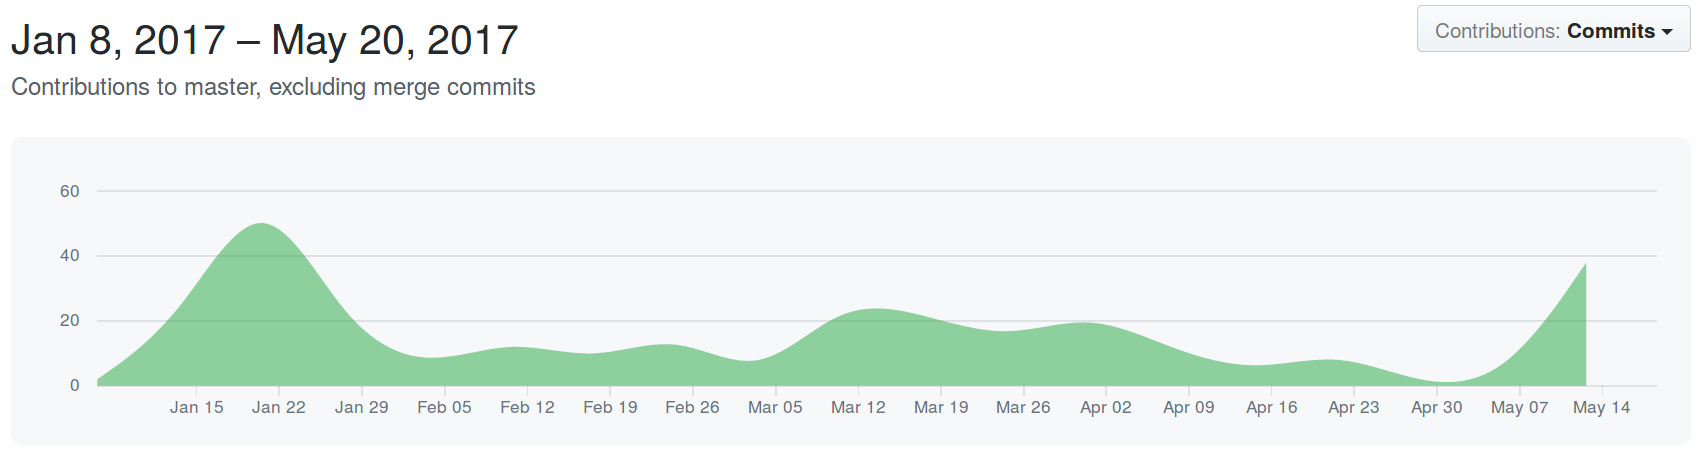
\includegraphics[width=1.0\textwidth]{images/temps.png}
\caption{R�partition des commits Git au cours du temps}
\label{fig:modele}
\end{figure}



\section{Conclusion}
\label{sec:conclusion}

\noindent Dans cette section, nous r�sumons la r�alisation du projet et nous pr�sentons �galement les extensions et am�liorations possibles du projet.


\listoffigures
\listoftables

%R�f�rences bibliographiques du document
\bibliographystyle{plain}
\bibliography{bibliographies}
\nocite{*}

\end{document}
